\chapter{Vector Basics}
    \section{Recommended Texts}
        The following books are recommended for the course. The first one will be followed by the instructor.
        \begin{enumerate}
            \item Engineering Electromagnetics 8th Edition by John Buck \& William H. Hayt
            \item Electromagnetics John D. Kraus
            \item Introduction to Electrodynamics by David J. Griffiths
            \item Classical Electrodynamics by John David Jackson
        \end{enumerate}
    \section{What is a Vector?}
        From a mathematical standpoint a vector is an element of a vector space. From a physical point of view a vector is a quantity that requires a magnitude as well as a direction to be represented.
    \section{Unit vectors in Rectangular Coordinate System}
        In a Rectangular Coordinate System (RCS), a vector can be represented as a linear sum of three unit vectors, namely $\vec{a}_x$, $\vec{a}_y$ and $\vec{a}_z$. In case of two dimensions, $\vec{a}_z$ is not needed. This is also depicted in figure~\ref{fig:vectors}.
        \begin{figure}
            \centering
            \subfloat[A vector in two dimensions]{
                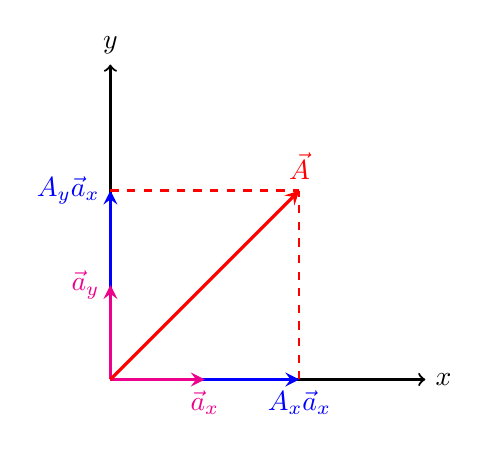
\begin{tikzpicture}
    [scale=4,
    axis/.style={->,thick},
    vector/.style={-stealth,very thick},
    vector guide/.style={dashed,red,thick}]

    \coordinate (O) at (0, 0);
    \def\u{0.3}
    \def\v{0.6}

    % drawing axes
    \draw[axis] (O) -- (1, 0) node[anchor=west]{$x$};
    \draw[axis] (O) -- (0, 1) node[anchor=south]{$y$};

    % drawing the vector's components
    \draw[vector, blue] (O) -- (\v, 0) node[anchor=north]{$A_x\vec{a}_x$};
    \draw[vector, blue] (O) -- (0, \v) node[anchor=east]{$A_y\vec{a}_x$};

    % drawing unit vectors
    \draw[vector, magenta] (O) -- (\u, 0) node[anchor=north]{$\vec{a}_x$};
    \draw[vector, magenta] (O) -- (0, \u) node[anchor=east]{$\vec{a}_y$};

    % drawing vector A
    \draw[vector, red] (O) -- (\v, \v) node[anchor=south]{$\vec{A}$};

    % drawing vector guides
    \draw[vector guide] (\v, 0) -- (\v, \v);
    \draw[vector guide] (0, \v) -- (\v, \v);

\end{tikzpicture}
            }
            \subfloat[A vector in three dimensions]{
                % sets up the perspective from which we are looking at the picture {theta}{phi}
% {theta} defines the rotion by x axis while {phi} defines the rotation by z axis
\tdplotsetmaincoords{60}{120}

\begin{tikzpicture}
    [scale=4,
    tdplot_main_coords,
    axis/.style={->,black,thick},
    vector/.style={-stealth,very thick},
    vector guide/.style={dashed,red,thick}]

    \coordinate (O) at (0, 0, 0);

    % this should serve as our unit vector
    \def\u{0.3} 
    \def\v{0.6}
    % drawing axes
    \draw[axis] (0, 0, 0) -- (1, 0, 0) node[anchor=north east]{$x$};
    \draw[axis] (0, 0, 0) -- (0, 1, 0) node[anchor=north west]{$y$};
    \draw[axis] (0, 0, 0) -- (0, 0, 1) node[anchor=south]{$z$};

    % drawing the components of the vector A: Drawing them first so the unit vectors do appear
    \draw[vector, blue] (O) -- (\v, 0, 0) node[anchor=south east]{$B_x\vec{a}_x$};
    \draw[vector, blue] (O) -- (0, \v, 0) node[anchor=south west]{$B_y\vec{a}_y$};
    \draw[vector, blue] (O) -- (0, 0, \v) node[anchor=south east]{$B_z\vec{a}_z$};

    % drawing the unit vectors
    \draw[vector, magenta] (O) -- (\u, 0, 0) node[anchor=south east]{$\vec{a}_x$};
    \draw[vector, magenta] (O) -- (0, \u, 0) node[anchor=south west]{$\vec{a}_y$};
    \draw[vector, magenta] (O) -- (0, 0, \u) node[anchor=east]{$\vec{a}_z$};

    % drawing the main vector B
    \draw[vector, red] (O) -- (\v, \v, \v) node[anchor=south east]{$\vec{B}$};

    % projection on xy axis
    \draw[vector guide] (\v, 0, 0) -- (\v, \v, 0);
    \draw[vector guide] (0, \v, 0) -- (\v, \v, 0);
    \draw [vector guide] (\v, \v, 0) -- (\v, \v, \v);

    % drawing projection on yz axis
    \draw[vector guide] (0, \v, 0) -- (0, \v, \v);
    \draw[vector guide] (0, 0, \v) -- (0, \v, \v);
    \draw[vector guide] (0, \v, \v) -- (\v, \v, \v);

    % drawing projection on xz axis
    \draw[vector guide] (0, 0, \v) -- (\v, 0, \v);
    \draw[vector guide] (\v, 0, 0) -- (\v, 0, \v);
    \draw[vector guide] (\v, 0, \v) -- (\v, \v, \v);


\end{tikzpicture}
            }
            \caption{}
            \label{fig:vectors}
        \end{figure}
    \section{Dot Product}
        Suppose we have two vectors $\vec{A}$ and $\vec{B}$. $\vec{A}$ can be represented as:
        $$\vec{A} = A_x\vec{a}_x + A_y\vec{a}_y + A_z\vec{a}_z$$
        Similarly, $\vec{B}$ can be represented as:
        $$\vec{B} = B_x\vec{a}_x + B_y\vec{a}_y + B_z\vec{a}_z$$
        Their dot product, $\vec{A}\cdot \vec{B}$, which is a scalar quantity, is defined as:
        \begin{equation}\label{eq:dotproductfirst}
            \vec{A}\cdot \vec{B} = |\vec{A}||\vec{B}|\cos \theta
        \end{equation}
        In case when $\theta$ becomes $90^{\circ}$ the dot product automatically reduces to zero. Thus one can easily conclude that the dot product of two perpendicular vectors shall always be zero. This makes expressing the dot product in terms of its components pretty straight forward.
        $$\vec{A}\cdot \vec{B} = \left(A_x\vec{a}_x + A_y\vec{a}_y + A_z\vec{a}_z\right)\cdot \left(B_x\vec{a}_x + B_y\vec{a}_y + B_z\vec{a}_z\right)$$
        \begin{equation}\label{eq:dotproduct}
           \vec{A}\cdot \vec{B} = A_xB_x + A_yB_y + A_zB_z
        \end{equation}
        A vector can also be represented in the form of column vector as:
        $$ \vec{A} = \begin{bmatrix}A_x \\A_y \\A_z\\ \end{bmatrix} \quad \vec{B} = \begin{bmatrix}B_x \\B_y \\B_z\\ \end{bmatrix} $$
        In that case the dot product, also called inner product in this context, is defined as:
        $$ \mathbf{A}^{T}\mathbf{B} $$
        If the vectors $\vec{A}$ and $\vec{B}$ are of the order $n \times 1$ their inner product will have the order $ 1 \times \left(n \times n\right) \times 1 = 1 \times 1$. Thus the result will be a scalar quantity.
        The opposite of the inner product is known as the outer product also called the cross product which we will get to in a later topic.
        
        \subsection{Cauchy Bunyakovsky Schwarz Inequality}
            The theorem states:
            $$|\vec{A}\cdot \vec{B}| \leq |\vec{A}||\vec{B}|$$
            It's easy to see why this is the case by replacing $\vec{A}\cdot \vec{B}$ by it's value:
            $$|\vec{A}||\vec{B}|\cos \theta \leq |\vec{A}||\vec{B}| $$
            This inequality changes to an equality when both vectors are collinear.
        
        \subsection{The Triangle Inequality}
            $$|\vec{A}| + |\vec{B}| \geq |\vec{A} + \vec{B}| $$
            It's quite easy to see why that is the case in the case of two dimensions.
            At this moment it should be useful to point out that:
            $$|\vec{A}| = \sqrt{A_x^2 + A_y^2 + A_z^2}$$
            $$|\vec{A}|^2 = \vec{A} \cdot \vec{A}$$
            This shall be useful in proving the Parallelogram Equality.
        
        \subsection{The Parallelogram Equality}
            The equality states:
            $$|\vec{A} + \vec{B}|^2 + |\vec{A} - \vec{B}|^2 = 2\left(|\vec{A}|^2+\vec{B}^2\right)$$
            To prove it:
            $$|\vec{A} + \vec{B}|^2 = \left(\vec{A}+\vec{B}\right)\cdot \left(\vec{A}+\vec{B}\right)$$
            $$= \vec{A}\cdot \vec{A} + \vec{A}\cdot \vec{B} + \vec{B}\cdot \vec{A} + \vec{B}\cdot \vec{B}$$
            $$= |\vec{A}|^2 -2\vec{A}\cdot \vec{B} + |\vec{B}|^2$$
            Similarly:
            $$|\vec{A} - \vec{B}|^2 = \left(\vec{A}-\vec{B}\right)\cdot \left(\vec{A}-\vec{B}\right)$$
            $$= \vec{A}\cdot \vec{A} - \vec{A}\cdot \vec{B} - \vec{B}\cdot \vec{A} + \vec{B}\cdot \vec{B}$$
            $$= |\vec{A}|^2 +2\vec{A}\cdot \vec{B} + |\vec{B}|^2$$
            Thus:
            $$|\vec{A} + \vec{B}|^2 + |\vec{A} - \vec{B}|^2 = 2|\vec{A}| + 2|\vec{B}| = 2\left(|\vec{A}| + |\vec{B}|\right)$$
        
        \subsection{Scalar component of one vector in the direction of another}
            \begin{figure}
    \centering
    \begin{tikzpicture}
        [scale=6,
        axis/.style={->,thick},
        vector/.style={-stealth,very thick},
        vector guide/.style={dashed,red,thick}]

        \def\ang{45}

        \draw (0, 0) node[left]{$O$};
        % drawing both vectors and their angle's arc
        \draw[vector, blue] (0, 0) -- (0.5, 0) node[anchor=north]{$\vec{A}$};
        \draw[vector, red] (0, 0) -- (\ang: 0.5) node[anchor=south]{$\vec{B}$};
        \draw[black] (0.1, 0) arc (0:\ang:0.1);
        \draw (30: 0.1) node[right]{$\theta$};

        % dropping a perpendicular from B's tip to A
        \draw[dashed] (\ang: 0.5) -- ($(0,0)!(\ang: 0.5)!(1, 0)$) node[below]{$P$};

        % dropping a perpendicular from A's tip to B
        \draw[dashed] (0.5, 0) -- ($(0,0)!(0.5, 0)!(\ang: 0.5)$) node[left]{$Q$};

    \end{tikzpicture}
    \caption{Projections of two vectors $\vec{A}$ and $\vec{B}$ on each other.}
    \label{fig:projectiontwovectors}
\end{figure}
            Dot product can be really handy when we want to figure out the projection of one vector onto the direction of another vector. Refer to figure\ref{fig:projectiontwovectors}. The line $\bar{OP}$ is the projection of vector $\vec{B}$ in the direction of $\vec{A}$. Similarly, $\bar{OQ}$ is the projection of vector $\vec{A}$ in the direction of vector $\vec{B}$. Since the line from the tip of vector $\vec{B}$ to $P$ is perpendicular to the vector $\vec{A}$ and the line from the tip of $\vec{A}$ to point $Q$ is perpendicular to vector $\vec{B}$. We can apply trigonometry to find out these projections. 

            \noindent Let $B_A$ denote the projection of vector $\vec{B}$ in the direction of $\vec{A}$ and let $A_B$ denote the projection of $\vec{A}$ in the direction of $\vec{B}$. Applying trigonometry we get:
            $$B_A = |\vec{B}|\cos\theta$$
            $$A_B = |\vec{A}|\sin\theta$$
            Recalling the definition of a dot product from equation~\ref{eq:dotproductfirst} we can see:
            $$B_A = \frac{\vec{A}\cdot\vec{B}}{|\vec{A}|} = \vec{u}_A\cdot\vec{B}$$
            $$A_B = \frac{\vec{A}\cdot\vec{B}}{|\vec{B}|} = \vec{u}_B\cdot\vec{A}$$
        
        \subsection{Some practical applications}
            Some common places in Physics where you will find the dot product being applied are:
            \begin{itemize}
                \item The formulas for work done.
                        $$W = \vec{F}\cdot \vec{d}$$ 
                        $$dW = \vec{F}\cdot \vec{dl}$$
                        $$W = \int\limits_{L} \vec{F}\cdot \vec{dl}$$
                \item The forumulas for Electric and Magnetic flux.
                        $$\phi_E = \vec{E}\cdot \vec{A}$$
                        $$\phi_M = \vec{B}\cdot \vec{A}$$
                \item A third one I don't understand yet. Need to confirm this one.
                        $$Q = \iint\limits_{S}\vec{D}\cdot \vec{dS}$$
            \end{itemize}
    \section{Cross Product}
        \subsection{The Definition}
            The cross product of two vectors $\vec{A}$ and $\vec{B}$ is given by:
            \begin{equation}\label{eq:crossproduct}
                \vec{A}\times \vec{B} = |\vec{A}||\vec{B}|\sin\theta \vec{u}_N
            \end{equation}
            Where $\theta\in\left[0, \pi\right]$ and $\vec{u}_N$ is a vector given by the right hand rule where fingers should be curled from the direction of $\vec{A}$ to the direction of $\vec{B}$.
            Since the direction of the cross product is dictated by the right hand rule we can already see that it is not a commutative operation. More accurately:
            \begin{equation}\label{eq:commutativeincrossproduct}
                \vec{A}\times\vec{B} = - (\vec{B}\times\vec{A})
            \end{equation}
            
        \subsection{Geometric Significance}
            \begin{figure}
    \centering
    \begin{tikzpicture}
        [scale=4,
        axis/.style={->,thick},
        vector/.style={-stealth,very thick},
        vector guide/.style={dashed,red,thick}]

        % drawing both vectors and their angle's arc
        \draw[vector, blue] (0, 0) -- (0.5, 0) node[anchor=north]{$\vec{A}$};
        \draw[vector, red] (0, 0) -- (30: 0.5) node[anchor=south]{$\vec{B}$};
        \draw[black] (0.1, 0) arc (0:30:0.1);
        \draw (12: 0.2) node[anchor=east]{$\theta$};

        % drawing the other lines 
        \draw[black, very thick] (30: 0.5) -- ++(0.5, 0);
        \draw[black, very thick] (0.5, 0) -- ++(30: 0.5);

        % height of the parallelogram
        \draw[dashed] (30:0.5) -- node[left]{$h$} ($(0,0)!(30:0.5)!(1,0)$);
    \end{tikzpicture}
    \caption{A parallelogram formed by two vectors $\vec{A}$ and $\vec{B}$}
    \label{fig:parallelogram}
\end{figure}
            As you can see very clearly in figure~\ref{fig:parallelogram} that any two vectors $\vec{A}$ and $\vec{B}$ can uniquely identify a parallelogram. The area of any parallelogram is given by the formula:
            \begin{equation}\label{eq:areaofparallelogram}
            Area = (base)\times(height)
            \end{equation}
            In figure~\ref{fig:parallelogram} the base is the length of the vector $\vec{A}$ and the height is shown by the dotted line. But how do we figure out what $h$ really is? By applying trigonometry here we can find out that $h = |\vec{A}|\sin\theta$. Plugging in these values in equation~\ref{eq:areaofparallelogram} we get:
            $$Area = (|\vec{B}|)(|\vec{A}|\sin\theta)$$
            Ahah, this is exactly the same formula that is given by $\vec{A}\cdot\vec{B}$. Thus we can conclude that the area of the parallelogram formed by two vectors $\vec{A}$ and $\vec{B}$ is given by $\vec{A}\cdot\vec{B}$.
            $$Area = \vec{A}\cdot\vec{B}$$
        
        \subsection{Calculating Cross Product}
            Before we learn how to calculate the cross product of any two vectors in terms of the three basic unit vectors $\vec{a}_x$, $\vec{a}_y$ and $\vec{a}_z$ we should think about what will be the cross production of every possible combination of two of these three unit vectors. We know from equation~\ref{eq:crossproduct} that the cross product of two parallel vectors should be zero because $\sin 90^{\circ} = 0$. We also know that the magnitude of a unit vector is by definition one. Using these two facts, along with the right hand rule, we can very quickly see that:
            $$\vec{a}_x\times\vec{a}_y=\vec{a}_z$$
            $$\vec{a}_y\times\vec{a}_z=\vec{a}_x$$
            $$\vec{a}_z\times\vec{a}_x=\vec{a}_y$$
            Using equation~\ref{eq:commutativeincrossproduct} we can easily figure out the reverses of these combinations:
            $$\vec{a}_y\times\vec{a}_x=-\vec{a}_z$$
            $$\vec{a}_z\times\vec{a}_y=-\vec{a}_x$$
            $$\vec{a}_x\times\vec{a}_z=-\vec{a}_y$$
            Now suppose we have two vectors $\vec{A}$ and $\vec{B}$, we can express them as:
            $$\vec{A} = A_x\vec{a}_x + A_y\vec{a}_y + A_z\vec{a}_z$$
            $$\vec{B} = B_x\vec{a}_x + B_y\vec{a}_y + B_z\vec{a}_z$$
            Their cross product can be written as:
            $$\vec{A}\times\vec{B} = \left(A_x\vec{a}_x + A_y\vec{a}_y + A_z\vec{a}_z\right)\times\left(B_x\vec{a}_x + B_y\vec{a}_y + B_z\vec{a}_z\right)$$
            Expanding this we get:
            \begin{align*}
            \vec{A}\times\vec{B} = A_xB_x(\vec{a}_x\times\vec{a}_x) + A_xB_y(\vec{a}_x\times\vec{a}_y) + A_xB_z(\vec{a}_x\times\vec{a}_z)\\ + A_yB_x(\vec{a}_y\times\vec{a}_x) + A_yB_y(\vec{a}_y\times\vec{a}_y) + A_yB_z(\vec{a}_y\times\vec{a}_z)\\ + A_zB_x(\vec{a}_z\times\vec{a}_x) + A_zB_y(\vec{a}_z\times\vec{a}_y) + A_zB_z(\vec{a}_z\times\vec{a}_z)
            \end{align*}
            Firstly, we can cancel those cross products which are between collinear vectors, as we know that's going to be zero.
            \begin{align*}
            \vec{A}\times\vec{B} = A_xB_y(\vec{a}_x\times\vec{a}_y) + A_xB_z(\vec{a}_x\times\vec{a}_z)\\ + A_yB_x(\vec{a}_y\times\vec{a}_x)  + A_yB_z(\vec{a}_y\times\vec{a}_z)\\ + A_zB_x(\vec{a}_z\times\vec{a}_x) + A_zB_y(\vec{a}_z\times\vec{a}_y) 
            \end{align*}
            Now, just utilizing the crossproducts of all possible combinations between unit vectors that we just derived a while ago, we can simplify this even further:
            \begin{align*}
            \vec{A}\times\vec{B} = A_xB_y(\vec{a}_z) + A_xB_z(-\vec{a}_y)\\ + A_yB_x(-\vec{a}_z)  + A_yB_z(\vec{a}_x)\\ + A_zB_x(\vec{a}_y) + A_zB_y(-\vec{a}_x) 
            \end{align*}
            Grouping these terms by unit vectors we get:
            \begin{equation}
                \vec{A}\times\vec{B} = \vec{a}_x(A_yB_z-A_zB_y) + \vec{a}_y(A_zB_x-A_xB_z) + \vec{a}_z(A_xB_y-A_yB_x)
            \end{equation}
            We can write this in an elegant way as a determinant:
            \begin{equation}
                \vec{A}\times\vec{B} = \begin{vmatrix}
                    \vec{a}_x & \vec{a}_y & \vec{a}_z \\
                    A_x & A_y & A_z\\
                    B_x & B_y & B_z
                \end{vmatrix}
            \end{equation}
        \subsection{Properties}
            Cross Product does not follow the commutative law as we have already seen. However, it does follow distributive law:
            $$\vec{A}\times\left(\vec{B}+\vec{C}\right) = \vec{A}\times\vec{B} + \vec{A}\times\vec{C}$$
        \subsection{Practical Applications}
            \begin{enumerate}
                \item Torque: $$\vec{\tau}=\vec{r}\times\vec{F}$$
                \item Angular Momentum: $$\vec{L}=\vec{r}\times\vec{\rho}$$ $$\vec{\rho}=m\vec{v}$$
                \item Force on a moving conductor: $$\vec{F} = I\vec{L}\times\vec{B}$$
                \item Force on a moving charge: $$\vec{F} = q\vec{v}\times\vec{B}$$
                \item Lorrentz Force Formula: $$\vec{F}=q\left(\vec{E}+\vec{v}\times\vec{B}\right)$$
            \end{enumerate}
    \section{Scalar Triple Product}
        \subsection{Definition}
            The Scalar Triple Product of three vectors $\vec{A}$, $\vec{B}$ and $\vec{C}$ is defined as:
            $$\vec{A}\cdot\left(\vec{B}\times\vec{C}\right)$$
            We already know that:
            \begin{equation}\label{eq:BintoC}
                \vec{B}\times\vec{C} = \begin{vmatrix}\vec{a}_x & \vec{a}_y & \vec{a}_z \\ B_x & B_y & B_z \\ C_x & C_y & C_z \end{vmatrix}
            \end{equation}
            Vector $\vec{A}$ is defined as:
            $$\vec{A} = A_x\vec{a}_x + A_y\vec{a}_y + A_z\vec{a}_z$$
            We also know from equation~\ref{eq:dotproduct} that when the dot product of two vectors is taken, their respective components are mulitplied together, the unit vectors go away and the resultant values are added, right?
            Let $\vec{V}$ represent $\vec{B}\times\vec{C}$. So, $\vec{A}\cdot\vec{V}$ is:
            $$\vec{A}\cdot\vec{V} = A_xV_x + A_yV_y + A_zV_z$$
            From equation~\ref{eq:BintoC} we can see that:
            $$V_x = \begin{vmatrix}B_y & B_z \\ C_y & C_z\end{vmatrix}$$
            $$V_y = -\begin{vmatrix}B_x & B_z \\ C_x & C_z\end{vmatrix}$$
            $$V_z = \begin{vmatrix}B_x & B_y \\ C_x & C_y\end{vmatrix}$$
            Putting these results back we get:
            $$\vec{A}\cdot\vec{V} = A_x\begin{vmatrix}B_y & B_z \\ C_y & C_z\end{vmatrix} + -A_y\begin{vmatrix}B_x & B_z \\ C_x & C_z\end{vmatrix} + \begin{vmatrix}B_x & B_y \\ C_x & C_y\end{vmatrix}$$ 
            Ahah, we have seen something similar while expanding determinants haven't we?
            \begin{equation}\label{eq:scalartriple}
            \vec{A}\cdot\left(\vec{B}\times\vec{C}\right) = \begin{vmatrix}A_x & A_y & A_z\\ B_x & B_y & B_z\\ C_x & C_y & C_z\end{vmatrix}
            \end{equation}
            Exchanging two rows of a determinant two times doesn't really doesn't affect it, right? That fact, leads to the equality:
            $$\vec{B}\cdot\left(\vec{C}\times\vec{A}\right) = \vec{C}\cdot\left(\vec{A}\times\vec{B}\right)$$
            % TODO: Must check this with instructor
            Another property that these follow is:
            $$\vec{A}\cdot\left(\vec{B}\times\vec{C}\right) = \vec{B}\left(\vec{C}\times\vec{A}\right) = \vec{C}\left(\vec{A}\times\vec{B}\right)$$
        \subsection{Applications}
            \subsubsection{Volume of Parallelopiped}
                % sets up the perspective from which we are looking at the picture {theta}{phi}
% {theta} defines the rotion by x axis while {phi} defines the rotation by z axis
\tdplotsetmaincoords{60}{45}
\begin{figure}
    \centering
    \begin{tikzpicture}
        [scale=3,
        tdplot_main_coords,
        axis/.style={->,black,thick},
        vector/.style={-stealth,very thick},
        vector guide/.style={dashed,red,thick}]

        \coordinate (O) at (0, 0, 0);
        \coordinate (A) at (1, 0, 0);
        \coordinate (B) at (0, 1, 0);
        \coordinate (C) at (0.5, 0.5, 1);

        \draw[vector, red] (O) -- node[below]{$\vec{A}$}(A);
        \draw[vector, blue] (O) -- node[above]{$\vec{B}$}(B);
        \draw[vector, green] (O) -- node[above]{$\vec{C}$}(C);

        % completing the parallelogram
        \draw (A) -- +(B);
        \draw (B) -- +(A);
        \draw (C) -- +(A);
        \draw (A) -- (1.5, 0.5, 1);
        \draw (B) -- +(C);
        \draw ($ (B) + (A) $) -- +(C);
        \draw ($ (B) + (A) + (C) $) -- ($ (B) + (C) $);
        \draw (C) -- +(B);
        \draw ($ (A) + (C) $) -- +(B);

        \draw[vector] (O) -- node[left]{$\vec{B}\times\vec{C}$} (0, 0, 1);

        \tdplotdefinepoints(0,0,0)(0, 0, 1)(0.5, 0.5, 1);
        \tdplotdrawpolytopearc[<->]{0.3}{above}{$\theta$}
    \end{tikzpicture}
    \caption{The parallelopiped formed by $\vec{A}$, $\vec{B}$ and $\vec{C}$}
    \label{fig:parallelopiped}
\end{figure}
                The area of a parallelopiped can be calculated by the following formula:
                $$Area = (\textrm{area of base face})\times(h)$$
                Where $h$ is the perpendicular distance between the base face and the top face.
                In figure~\ref{fig:parallelopiped} we can see that a parallelopiped is uniquely identified by three vectors $\vec{A}$, $\vec{B}$ and $\vec{C}$. The area of the base face, as we already know, is given by the magnitude of the cross product of $\vec{A}$ and $\vec{B}$. The vector $\vec{A}\times\vec{B}$ is also shown in figure~\ref{fig:parallelopiped}. The magnitude of this vector gives us the area and direction of this vector is perpendicular to the plane formed by $\vec{A}$ and $\vec{B}$. Now we need to figure out the perpendicular distance between the base face and the top face. That distance is given by $|\vec{C}|\cos\theta$. If we take the dot product of $\vec{A}\times\vec{B}$ and $\vec{C}$ we get:
                \begin{align*}
                    \vec{C}\cdot\left(\vec{A}\times\vec{B}\right) = \left(|\vec{C}|\cos\theta\right)\left(|\vec{A}\times\vec{B}|\right)\\ 
                    = \left(|\vec{C}|\cos\theta\right)\left(\textrm{area of base face}\right)\\
                    = \left(\textrm{h}\right)\left(\textrm{area of base face}\right)\\
                    = \textrm{Volume of the parallelopiped}
                \end{align*}
                Hence we have proven that the scalar product of three vectors gives us the volume of the parallelopiped formed by them.
            \subsubsection{Volume of a Tetrahedron}
                % sets up the perspective from which we are looking at the picture {theta}{phi}
% {theta} defines the rotion by x axis while {phi} defines the rotation by z axis
\tdplotsetmaincoords{60}{70}
\begin{figure}
    \centering
    \begin{tikzpicture}
        [scale=3,
        tdplot_main_coords,
        axis/.style={->,black,thick},
        vector/.style={-stealth,very thick},
        vector guide/.style={dashed,red,thick}]

        \coordinate (O) at (0, 0, 0);
        \coordinate (A) at (1, 0, 0);
        \coordinate (B) at (0, 1, 0);
        \coordinate (C) at (0.3, 0.3, 1);

        \draw[vector, red] (O) -- node[left]{$\vec{A}$}(A);
        \draw[vector, blue] (O) -- node[above]{$\vec{B}$}(B);
        \draw[vector, green] (O) -- node[right]{$\vec{C}$}(C);

        \draw (A) -- (B);
        \draw (A) -- (C);
        \draw (B) -- (C);
        \draw[dashed] (O) -- node[left]{$h$} ($(O)!(C)!(0, 0, 1)$);

        \draw[dotted] (A) -- ($(A)+(B)$);
        \draw[dotted] (B) -- ($(B)+(A)$);

        \tdplotdefinepoints(0,0,0)(1, 0, 0)(0, 1, 0);
        \tdplotdrawpolytopearc[<->]{0.3}{below}{$\theta$}


        \tdplotdefinepoints(0,0,0)(0, 0, 1)(0.3, 0.3, 1);
        \tdplotdrawpolytopearc[<->]{0.4}{above}{$\phi$}
    \end{tikzpicture}
    \caption{The Tetrahedron formed by $\vec{A}$, $\vec{B}$ and $\vec{C}$}
    \label{fig:tetrahedron}
\end{figure}
                A tetrahedron is uniquely identified by three vectors $\vec{A}$, $\vec{B}$ and $\vec{C}$. Figure~\ref{fig:tetrahedron} represents one such tetrahedron. The area of a tetrahedron is given by the following formula:
                $$\left(\textrm{Area of a tetrahedron}\right)=\left(\textrm{Area of base}\right)\times(h)$$
                We can see in figure~\ref{fig:tetrahedron} that:
                $$\textrm{Area of base} = \frac{1}{2}\times\textrm{Area of the parallelogram formed by }\vec{A}, \vec{B}$$
                We also know from the previous sections that:
                $$\textrm{Area of the parallelogram formed by }\vec{A}, \vec{B} = |\vec{A}||\vec{B}|\sin\theta$$
                We can see from figure~\ref{fig:tetrahedron} that:
                $$h = |\vec{C}|\cos\phi$$
                Thus the total volume is given by:
                $$\textrm{Volume} = \frac{1}{3}\left(\frac{1}{2}|\vec{A}||\vec{B}|\sin\theta\right)\left(|\vec{C}|\cos\phi\right)$$
                $$\textrm{Volume} = \frac{1}{6}\left(\vec{A}\times\vec{B}\right)\cdot\vec{C}$$
    \section{Vector Triple Product}
        It is defined as: $$\vec{A}\times \left(\vec{B}\times\vec{C}\right)$$
        This can be evaluated by triple product expansion also known as `Lagrange\'s formula' which is:
        $$\vec{B}\left(\vec{A}\times\vec{C}\right) - \vec{C}\left(\vec{A}\cdot\vec{B}\right)$$
        It can also be represented as `BAC - CAP'.
    \section{Coordinate Systems}
        We will be dealing with three coordinate systems in this development:
        \begin{enumerate}
            \item Rectangular Coordinate System (RCS)
            \item Cylindrical Coordinate System (CCS)
            \item Spherical Coordinate System (SCS)
        \end{enumerate}
        \subsection{Rectangular Coordinate System}
            % sets up the perspective from which we are looking at the picture {theta}{phi}
% {theta} defines the rotion by x axis while {phi} defines the rotation by z axis
\tdplotsetmaincoords{60}{120}
\begin{figure}
    \centering
    \begin{tikzpicture}
        [scale=4,
        tdplot_main_coords,
        axis/.style={->,black,thick},
        vector/.style={-stealth,very thick},
        vector guide/.style={dashed,red,thick}]

        \coordinate (O) at (0, 0, 0);

        % this should serve as our unit vector
        \def\u{0.3} 
        \def\v{0.6}
        % drawing axes
        \draw[axis] (0, 0, 0) -- (1, 0, 0) node[anchor=north east]{$x$};
        \draw[axis] (0, 0, 0) -- (0, 1, 0) node[anchor=north west]{$y$};
        \draw[axis] (0, 0, 0) -- (0, 0, 1) node[anchor=south]{$z$};

        % drawing the unit vectors
        \draw[vector, magenta] (O) -- node[anchor=south east]{$\vec{a}_x$} (\u, 0, 0);
        \draw[vector, magenta] (O) -- node[anchor=south]{$\vec{a}_y$} (0, \u, 0);
        \draw[vector, magenta] (O) -- node[anchor=east]{$\vec{a}_z$} (0, 0, \u);

        % drawing the main vector B
        \fill[red] (\v, \v, 1) circle[radius=0.6pt] node[right]{$P$};

        % projection on xy axis
        \draw[vector guide] (\v, 0, 0) -- node[below]{$P_x$}(\v, \v, 0);
        \draw[vector guide] (0, \v, 0) -- node[below]{$P_y$}(\v, \v, 0);
        \draw [vector guide] (\v, \v, 0) -- node[right]{$P_z$}(\v, \v, 1);

    \end{tikzpicture}
    \caption{A point $P$ in Rectangular Coordinate Systems}
    \label{fig:point-rcs}
\end{figure}
            A point in RCS as shown in figure~\ref{fig:point-rcs} is represented by three coordinates $\left(x, y, z\right)$ each representing the distance along that particular axis as shown in the figure. RCS has three unit vectors $\vec{a}_x$, $\vec{a}_y$ and $\vec{a}_z$.
        \subsection{Cylindrical Coordinate System}
            % sets up the perspective from which we are looking at the picture {theta}{phi}
% {theta} defines the rotion by x axis while {phi} defines the rotation by z axis
\begin{figure}
    \tdplotsetmaincoords{60}{120}
    \centering
    \begin{tikzpicture}
        [scale=4,
        tdplot_main_coords,
        axis/.style={->,black,thick},
        vector/.style={-stealth,very thick},
        vector guide/.style={dashed,red,thick}]
        
        % defines unit vector length
        \def\unit{0.3}

        % defines the x, y, and z coordinates for point P
        \def\ax{0.5}
        \def\ay{0.5}
        \def\az{0.5}

        \coordinate (O) at (0, 0, 0); % denote origin by (O)
        \coordinate (P) at (\ax, \ay, \az); % denote point P by (P)

        \def\rholength{ {sqrt(\ax^2+\ay^2)} } % \rholength stores the distance between Pxy and O

        % these should serve as our axes
        \draw[axis] (0, 0, 0) -- (1, 0, 0) node[anchor=north east]{$x$};
        \draw[axis] (0, 0, 0) -- (0, 1, 0) node[anchor=north west]{$y$};
        \draw[axis] (0, 0, 0) -- (0, 0, 1) node[anchor=south]{$z$};

        \draw[blue] (O) -- node[right]{$\rho$} (\ax, \ay, 0); % draws rho line
        \draw[dashed] (\rholength, 0, 0) arc (0:90:\rholength); % draws the circle r=rho on xy plane
        \draw[red] (P) -- node[right]{$z$} (\ay, \ay, 0); % line between point P and its xy plane projection

        \fill[red] (P) circle[radius=0.5pt] node[right]{$P(\rho, \phi, z)$}; % point P as a filled circle

        % drawing the arc of the angle between rho and x axis
        \tdplotdefinepoints(0,0,0)(1, 0, 0)(\ax, \ax, 0); 
        \tdplotdrawpolytopearc[-]{0.2}{below}{$\phi$}

        % setting up some lengths for drawing unit vectors
        \def\unitvectorrhox{ {\unit*cos{45}} }
        \def\unitvectorrhoy{ {\unit*sin{45}} }

        \def\unitvectorphix{ {\unit*cos{135}} }
        \def\unitvectorphiy{ {\unit*sin{135}} }

        \draw[vector, red] (O) -- (0, 0, \unit) node[right]{$\vec{a}_z$}; % unit vector az
        \draw[vector, blue] (O) -- node[right, yshift=10]{$\vec{a}_\rho$} (\unitvectorrhox, \unitvectorrhoy, 0); % unit vector a\rho
        \draw[vector] (0.5, 0.5, 0) -- node[below]{$\vec{a}_\phi$} +(\unitvectorphix, \unitvectorphiy, 0); % unit vector a\phi

    \end{tikzpicture}
    \caption{A point $P$ represented in CCS}
    \label{fig:pointinccs}
\end{figure}
            A point in CCS, as depicted in figure~\ref{fig:pointinccs}, is represented by three coordinates $\left(\rho, \phi, z\right)$ where $\rho \in [0, \infty)$ and $\phi \in [0, 2\pi]$. $\rho$ is the distance between the origin and the point's projection on the $xy$ plane. $\phi$ is the angle between the x-axis and the $\rho$ line. $z$ is the distance between the point and it's projection on the $xy$ plane. The three unit vectors in this coordinate system are $\vec{a}_\rho$, $\vec{a}_\phi$ and $\vec{a}_z$. $\vec{a}_z$ is the same as in RCS. $\vec{a}_\rho$ takes the direction along the $\rho$ line, and $\vec{a}_\phi$ takes the direction of increasing $\phi$.
            
            Let's write out the equations to convert $(x, y, z)$ to $(\rho, \phi, z)$ and back.
            \begin{align}
                x = \rho\cos\phi \\
                y = \rho\sin\phi \\
                z = z
            \end{align}
            \begin{align}
                \rho = \sqrt{x^2+y^2} \\
                \phi = \tan^{-1}\phi
            \end{align}

            Let's now try and write the equations to represent the unit vectors $\vec{a}_\rho$, $\vec{a}_\phi$ in terms of $\vec{a}_x$, $\vec{a}_y$ and $\vec{a}_z$ respectively. $\vec{a}_z$ doesn't need to be converted since its the same on both sides.
            We call the vector from the origin to the point's projection on xy axis $\vec{\rho}$. $\vec{\rho}$ can be written as:
            $$\vec{\rho} = \rho\cos\phi\vec{a}_x + \rho\sin\phi\vec{a}_y$$
            $$|\vec{\rho}| = \rho$$
            Thus we can write:
            $$\vec{a}_\rho = \cos\phi\vec{a}_x + \sin\phi\vec{a}_y$$
            We can see that $\vec{a}_\phi$ is the cross product of $\vec{a}_z$ and $\vec{a}_\rho$:
            $$\vec{a}_\phi = \vec{a}_z\times\vec{a}_\rho$$
            \begin{align}
                \vec{a}_\rho = \cos\phi\vec{a}_x + \sin\phi\vec{a}_y + 0\vec{a}_z \\ 
                \vec{a}_\phi = -\sin\phi\vec{a}_x + \cos\phi\vec{a}_y + 0\vec{a}_z \\
                \vec{a}_z = 0\vec{a}_x + 0\vec{a}_y + \vec{a}_z
            \end{align}
            Writing this in an elegant form:
            \begin{equation}\label{eq:rcstoccsunit}
                \begin{bmatrix}
                    \vec{a}_\rho \\ \vec{a}_\phi \\ \vec{a}_z 
                \end{bmatrix} = 
                \begin{bmatrix}
                    \cos\phi & \sin\phi & 0 \\
                    -\sin\phi & \cos\phi & 0 \\
                    0 & 0 & 1
                \end{bmatrix}
                \begin{bmatrix}
                    \vec{a}_x \\
                    \vec{a}_y \\
                    \vec{a}_z
                \end{bmatrix}
            \end{equation}
            This can be summarized as:
            $$\vec{u}_c = T\left(\phi\right)\vec{u}_R$$
            Where $T\left(\phi\right)$ is the transformation written as a function of $\phi$. To find the reverse transformation we can take the inverse of this transformation matrix. But we should note that this transformation is what is called an Orthogonal Transformation. In an Orthogonal Transformation the inverse transformation matrix is given by taking the transpose of the transformation matrix. Thus:
            \begin{equation}
                \begin{bmatrix}
                    \vec{a}_x \\ \vec{a}_y \\ \vec{a}_z
                \end{bmatrix} = 
                \begin{bmatrix}
                    \cos\phi & -\sin\phi & 0 \\
                    \sin\phi & \cos\phi & 0 \\
                    0 & 0 & 1
                \end{bmatrix}
                \begin{bmatrix}
                    \vec{a}_\rho \\
                    \vec{a}_\phi \\
                    \vec{a}_z
                \end{bmatrix}
            \end{equation}

            A vector $\vec{A}$ can be represented in RCS as:
            \begin{equation}\label{eq:vectorAinRCS}
                \vec{A} = A_x\vec{a}_x = A_y\vec{a}_y + A_z\vec{a}_z
            \end{equation}
            The same vector can be represented in CCS as:
            $$\vec{A} = A_\rho\vec{a}_\rho + A_\phi\vec{a}_\phi + A_z\vec{a}_z$$
            Let's try to write a relationship between $A_\rho$, $A_\phi$ and $A_z$ in terms of $A_x$, $A_y$ and $A_z$.
            We start with the equation:
            $$\vec{A} = A_\rho\vec{a}_\rho + A_\phi\vec{a}_\phi + A_z\vec{a}_z$$
            We try to replace $\vec{a}_\rho$, $\vec{a}_\phi$ with their RCS counterparts by using equation~\ref{eq:rcstoccsunit}.
            \begin{align*}
                \vec{A} = A_\rho\left(\cos\phi\vec{a}_x + \sin\phi\vec{a}_y\right) + \\
                          A_\phi\left(-\sin\phi\vec{a}_x + \cos\phi\vec{a}_y\right) + \\
                          A_z\vec{a}_z
            \end{align*}
            Grouping the terms in the above equation by unit vectors we get:
            \begin{align*}
                \vec{A} =  + \vec{a}_x\left(A_\rho\cos\phi - A_\phi\sin\phi\right)\\
                           + \vec{a}_y\left(A_\rho\sin\phi + A_\phi\cos\phi\right)\\
                           + A_z\vec{a}_z
            \end{align*}
            Thus comparing this with equation~\ref{eq:vectorAinRCS} we can conclude:
            \begin{align*}
                A_x = A_\rho\cos\phi - A_\phi\sin\phi\\
                A_y = A_\rho\sin\phi + A_\phi\cos\phi\\
                A_z = A_z
            \end{align*}
            We can write this in an elegant way as:
            \begin{equation}
                \begin{bmatrix}
                    A_x \\ A_y \\ A_z
                \end{bmatrix}
                =
                \begin{bmatrix}
                    \cos\phi & -\sin\phi & 0 \\
                    \sin\phi & \cos\phi & 0 \\
                    0 & 0 & 1
                \end{bmatrix}
                \begin{bmatrix}
                    A_\rho \\ A_\phi \\ A_z
                \end{bmatrix}
            \end{equation}
            Since this transformation is orthogonal too we can find the inverse relationship by simply taking the transpose of the transformation matrix:
            \begin{equation}
                \begin{bmatrix}
                    A_\rho \\ A_\phi \\ A_z
                \end{bmatrix}
                =
                \begin{bmatrix}
                    \cos\phi & \sin\phi & 0 \\
                    -\sin\phi & \cos\phi & 0 \\
                    0 & 0 & 1
                \end{bmatrix}
                \begin{bmatrix}
                    A_x \\ A_y \\ A_z
                \end{bmatrix}
            \end{equation}
        \subsection{Spherical Coordinate Systems}
            \begin{figure}
    \tdplotsetmaincoords{60}{120}
    \centering
    \begin{tikzpicture}
        [scale=4,
        tdplot_main_coords,
        axis/.style={->,black,thick},
        vector/.style={-stealth,very thick},
        vector guide/.style={dashed,red,thick}]

        % defines unit vector length
        \def\unit{0.3}

        % define our point P in spherical coordiantes
        \def\r{0.6}
        \def\phiii{80}
        \def\thetaaa{45}

        % defines the x, y, and z coordinates for point P
        \def\ax{ {\r*sin(\thetaaa)*cos(\phiii)} }
        \def\ay{ {\r*sin(\thetaaa)*sin(\phiii)} }
        \def\az{ {\r*cos(\thetaaa)} }

        \coordinate (O) at (0, 0, 0); % denote origin by (O)
        \coordinate (P) at (\ax, \ay, \az); % denote point P by (P)

        \def\rholength{ {sqrt(\ax^2+\ay^2)} } % \rholength stores the distance between Pxy and O


        % these should serve as our axes
        \draw[axis] (0, 0, 0) -- (1, 0, 0) node[anchor=north east]{$x$};
        \draw[axis] (0, 0, 0) -- (0, 1, 0) node[anchor=north west]{$y$};
        \draw[axis] (0, 0, 0) -- (0, 0, 1) node[anchor=south]{$z$};

        \draw[blue] (O) -- node[right]{$\rho$} (\ax, \ay, 0); % draws rho line
        % \draw[dashed] (\rholength, 0, 0) arc (0:90:\rholength); % draws the circle r=rho on xy plane
        \draw[red, dashed] (P) -- (\ax, \ay, 0); % line between point P and its xy plane projection

        \draw[black] (O) -- (P); % drawing the r part

        \fill[red] (P) circle[radius=0.5pt] node[right]{$P(r, \phi, \theta)$}; % point P as a filled circle

        % drawing the arc of the angle between rho and x axis
        \tdplotdefinepoints(0,0,0)(1,0,0)(\ax, \ay, 0)
        \tdplotdrawpolytopearc[-]{0.2}{below}{$\phi$}

        % create a theta plane basically
        \tdplotsetthetaplanecoords{\phiii}
        %draw theta arc and label, using rotated coordinate system
        \tdplotdrawarc[tdplot_rotated_coords]{(0,0,0)}{0.2}{0}{\thetaaa}{anchor=south west}{$\theta$}

    \end{tikzpicture}
    \caption{A point in Spherical Coordinate Systems}
    \label{fig:point-scs}
\end{figure}
            A point in spherical coordinate system can be represented as shown in figure~\ref{fig:point-scs}.
            In spherical coordinate system, a point is represented by three coordinates $(r,\phi,\theta)$. Here $r$ is the distance from the origin to the point itself. $\phi$ is the angle the point's projection on the xy-plane makes with the positive x axis. And finally $\theta$ is the angle the line from the origin to the point itself makes with the positive z axis. Two more conditions apply here:
            \begin{align*}
                \theta \in & \left[0,\pi\right]\\
                \phi \in & \left[0, 2\pi\right]
            \end{align*}
            Let's write the equations which can let us convert between spherical coordinates and rectangular coordinates.
            It is very easy to see in figure~\ref{fig:point-scs} that:
            \begin{align*}
                z = r\cos\theta\\
                \rho = r\sin\theta\\
                x = \rho\cos\phi\\
                y = \rho\sin\phi
            \end{align*}
            Thus we can write:
            \begin{align}
                z = r\cos\theta\\
                x = r\sin\theta\cos\phi\\
                y = r\sin\theta\sin\phi
            \end{align}
            We can do the reverse as:
            \begin{align}
                r = & \sqrt{x^2+y^2+z^2}\\
                \theta = & \tan^{-1}\left(\frac{\sqrt{x^2+y^2}}{z}\right)\\
                \theta = & \cos^{-1}\left(\frac{z}{\sqrt{x^2+y^2+z^2}}\right)\\
                \phi = & \tan^{-1}\left(\frac{y}{x}\right)
            \end{align}
            Now we need to express the unit vectors $(\vec{a}_r, \vec{a}_\phi, \vec{a}_\theta)$ in terms of $(\vec{a}_x, \vec{a}_y, \vec{a}_z)$. 
            Suppose we have a vector $\vec{r}$, and $r$ represents its magnitude. We can write it as:
            $$\vec{r} = x\vec{a}_x + y\vec{a}_y + z\vec{a}_z$$
            Dividing both sides by $r$ we get:
            $$\frac{\vec{r}}{r} = \frac{x}{r}\vec{a}_x + \frac{y}{r}\vec{a}_y + \frac{z}{r}\vec{a}_z$$
            Doing some substitutions we get:
            $$\vec{a}_r = \frac{r\sin\theta\cos\phi}{r}\vec{a}_x + \frac{r\sin\theta\sin\phi}{r}\vec{a}_y + \frac{r\cos\theta}{r}\vec{a}_z$$
            Simplifying we get:
            $$\vec{a}_r = \sin\theta\cos\phi\vec{a}_x + 
             \sin\theta\sin\phi\vec{a}_y +
             \cos\theta\vec{a}_z 
            $$
            We already know that:
            $$\vec{a}_\rho = \sin\phi\vec{a}_x + \cos\phi\vec{a}_y$$
            We can see in figure~\ref{fig:point-scs} that the vector $\vec{a}_\phi$ is at an angle $\phi + 90$ from the positive x axis. Thus putting in this angle we get:
            $$\vec{a}_\phi = \sin\left(\phi + 90\right)\vec{a}_x + \cos\left(\phi + 90\right)\vec{a}_y$$
            Using trigonometric identities we can get:
            $$\vec{a}_\phi = -\sin\phi\vec{a}_x + \cos\phi\vec{a}_y$$
            We can get $\vec{a}_\theta$ by realizing that:
            $$\vec{a}_\theta = \vec{a}_\phi \times \vec{a}_r$$
            Evaluating this $\vec{a}_\theta$:
            $$\vec{a}_\theta = 
                \begin{vmatrix}
                    \vec{a}_x & \vec{a}_y & \vec{a}_z \\
                    -\sin\phi & \cos\phi & 0 \\
                    \sin\theta\cos\phi & \sin\theta\sin\phi & \cos\theta 
                \end{vmatrix}$$
            Expanding this we get:
            $$
                \vec{a}_\theta = 
                \vec{a}_x\begin{vmatrix}
                    \cos\phi & 0 \\
                    \sin\theta\sin\phi & \cos\theta
                \end{vmatrix} - 
                \vec{a}_y\begin{vmatrix}
                   -\sin\phi & 0 \\
                   \sin\theta\cos\phi & \cos\theta 
                \end{vmatrix} + 
                \vec{a}_z\begin{vmatrix}
                   -\sin\phi & \cos\phi \\
                   \sin\theta\cos\phi & \sin\theta\sin\phi 
                \end{vmatrix}
            $$
            $$
                \vec{a}_\theta = \cos\theta\cos\phi\vec{a}_x
                + \sin\phi\cos\theta\vec{a}_y
                + \left(-sin^2\phi\sin\theta - \sin\theta\cos^2\phi\right)\vec{a}_z
            $$
            $$
                \vec{a}_\theta = \cos\theta\cos\phi\vec{a}_x
                + \sin\phi\cos\theta\vec{a}_y
                - \sin\theta\vec{a}_z
            $$
            Or more elegantly:
            $$\vec{a}_\theta = 
                \begin{bmatrix}
                    \cos\theta\cos\phi \\
                    \sin\phi\cos\theta \\
                    -\sin\theta
                \end{bmatrix}
            $$
            Or even more elegantly we can write:
            \begin{equation}
                \begin{bmatrix}
                    \vec{a}_r \\
                    \vec{a}_\theta \\
                    \vec{a}_\phi 
                \end{bmatrix} 
                =
                \begin{bmatrix}
                    \sin\theta\cos\phi & \sin\theta\sin\phi & \cos\theta \\
                    \cos\theta\cos\phi & \sin\phi\cos\theta & -\sin\theta \\
                    -\sin\phi & \cos\phi & 0
                \end{bmatrix}
                \begin{bmatrix}
                    \vec{a}_x \\
                    \vec{a}_y \\
                    \vec{a}_z 
                \end{bmatrix}
            \end{equation}
            Some useful relationships between these unit vectors are:
            \begin{align}
                \vec{a}_r \times \vec{a}_\theta & = \vec{a}_\phi \\
                \vec{a}_\theta \times \vec{a}_\phi & = \vec{a}_r \\
                \vec{a}_\phi \times \vec{a}_r & = \vec{a}_\theta 
            \end{align}
            Their reverses are easy to find. They will just have a negative sign.
            Suppose we have a vector $\vec{A}$. We can express it in terms of RCS as:
            $$\vec{A} = \vec{A}_x\vec{a}_x + \vec{A}_y\vec{a}_y + \vec{A}_z\vec{a}_z$$
            We can also express it in SCS as:
            $$\vec{A} = \vec{A}_r\vec{a}_r + \vec{A}_\theta\vec{a}_\theta + \vec{A}_\phi\vec{a}_\phi$$
            Let's replace $\vec{a}_r$, $\vec{a}_\theta$ and $\vec{a}_\phi$ in terms of $\vec{a}_x$, $\vec{a}_y$ and $\vec{a}_z$ using the matrix we just derived:
            \begin{align*}
                \vec{A} = & A_r\left(\sin\theta\cos\phi\vec{a}_x + \sin\theta\sin\phi\vec{a}_y + \cos\theta\vec{a}_z\right) \\
                & A_\theta\left(\cos\theta\cos\phi\vec{a}_x + \sin\phi\cos\theta\vec{a}_y -\sin\theta\vec{a}_z\right) \\ 
                & A_\phi\left(-\sin\phi\vec{a}_x + \cos\phi\vec{a}_y\right)
            \end{align*}
            Let's group these by the unit vectors $\vec{a}_x$, $\vec{a}_y$ and $\vec{a}_z$
            \begin{align*}
                \vec{A} = & \vec{a}_x \left(A_r\sin\theta\cos\phi + A_\theta\cos\theta\cos\phi - A_\phi\sin\phi\right)\\
                & \vec{a}_y \left(A_r\sin\theta\sin\phi + A_\theta\sin\phi\cos\theta + A_\phi\cos\phi\right) \\
                & \vec{a}_z \left(A_r\cos\theta - A_\theta\sin\theta\right)
            \end{align*}
            \begin{equation}
                \begin{bmatrix}
                    A_x \\ A_y \\ A_z    
                \end{bmatrix}
                =
                \begin{bmatrix}
                    \sin\theta\cos\phi & \cos\theta\cos\phi & -\sin\phi \\
                    \sin\theta\sin\phi & \cos\theta\sin\phi & \cos\theta \\
                    \cos\theta & -\sin\theta & 0
                \end{bmatrix}
                \begin{bmatrix}
                    A_r \\ A_\theta \\ A_\phi
                \end{bmatrix}
            \end{equation}
            Transposing this we get the inverse transformation:
            \begin{equation}
                \begin{bmatrix}
                    A_r \\ A_\theta \\ A_\phi    
                \end{bmatrix}
                =
                \begin{bmatrix}
                    \sin\theta\cos\phi & \sin\theta\sin\phi & \cos\theta \\
                    \cos\theta\cos\phi & \cos\theta\sin\phi & -\sin\theta \\
                    -\sin\phi & \cos\theta & 0
                \end{bmatrix}
                \begin{bmatrix}
                    A_x \\ A_y \\ A_z
                \end{bmatrix}
            \end{equation}
        \subsection{A little note about Orthogonal Transformations}
            Orthogonal transformations have this special property that their inverse transformation matrix is just the transpose of the orignal transformation matrix. This is why we have been able to just transpose the matrix and get the reverse transformation matrix. We have done this with RCS to CCS and CCS to RCS transformations and we just did it with RCS to SCS and SCS to RCS. 
            There are two types of orthogonal transformation matrix:
            \begin{itemize}
                \item Rotational Matrix (determinant $1$)
                \item Reflection Matrix (determinant $-1$)
            \end{itemize}
            We can prove that the determinant of an Orthogonal Transformation matrix is always either $1$ or $-1$ as:
            $$A^{-1} = A^T$$
            Let's do a right multiplication by $A$.
            $$A^{-1}A = A^TA$$
            $$I = A^TA$$
            Taking determinant on both sides:
            $$det(I) = det(A^T)det(A)$$
            $$1 = {det(A)}^2$$
            $$det(A) = \pm 1$$
    \section{Differential Lengths, Areas and Volumes}
        \subsection{RCS}
            % sets up the perspective from which we are looking at the picture {theta}{phi}
% {theta} defines the rotion by x axis while {phi} defines the rotation by z axis
\tdplotsetmaincoords{60}{120}
\begin{figure}
    \centering
    \begin{tikzpicture}
        [scale=4,
        tdplot_main_coords,
        axis/.style={->,black,thick},
        vector/.style={-stealth,very thick},
        vector guide/.style={dashed,red,thick}]

        \coordinate (O) at (0, 0, 0);

        % this should serve as our unit vector
        \def\unit{0.3} 

        \def\ax{0.4}
        \def\ay{0.5}
        \def\az{0.8}

        \def\bx{1}
        \def\by{1}
        \def\bz{1.2}

        \pgfmathsetmacro{\dx}{\bx-\ax}
        \pgfmathsetmacro{\dy}{\by-\ay}
        \pgfmathsetmacro{\dz}{\bz-\az}

        \pgfmathsetmacro{\dxd}{\dx/2}
        \pgfmathsetmacro{\dyd}{\dy/2}
        \pgfmathsetmacro{\dzd}{\dz/2}

        % drawing axes
        \draw[axis] (0, 0, 0) -- (1, 0, 0) node[anchor=north east]{$x$};
        \draw[axis] (0, 0, 0) -- (0, 1, 0) node[anchor=north west]{$y$};
        \draw[axis] (0, 0, 0) -- (0, 0, 1) node[anchor=south]{$z$};

        % drawing the main vector B
        \fill[red] (\ax, \ay, \az) circle[radius=0.2pt] node[right]{};
        \draw[vector, red] (0, 0, 0) -- (\ax, \ay, \az);

        \fill[blue] (\bx, \by, \bz) circle[radius=0.2pt] node[right]{};
        \draw[vector, blue] (0, 0, 0) -- (\bx, \by, \bz);

        \draw (\ax, \ay, \az) -- ++(\dx, 0, 0) -- ++(0, \dy, 0) -- node[right]{$dx$} ++(-\dx, 0, 0) -- ++(0, -\dy, 0);
        \draw (\ax, \ay, \az) -- ++(0, 0, \dz) -- ++(\dx, 0, 0) -- ++(0, \dy, 0) -- ++(-\dx, 0, 0) -- node[above]{$dy$} ++(0, -\dy, 0);
        \draw (\ax+\dx, \ay, \az) -- +(0, 0, \dz);
        \draw (\ax+\dx, \ay+\dy, \az) -- +(0, 0, \dz);
        \draw (\ax, \ay+\dy, \az) -- node[right]{$dz$} +(0, 0, \dz);

        % drawing the projections of red
        \draw[vector guide] (\ax, \ay, \az) -- (\ax, \ay, 0);
        \draw[vector guide] (\ax, 0, 0) -- (\ax, \by, 0);
        \draw[vector guide] (0, \ay, 0) -- (\bx, \ay, 0);

        % drawing the projections of blue
        \draw[vector guide, blue] (\bx, \by, \bz-\dz) -- (\bx, \by, 0);
        \draw[vector guide, blue] (\bx, 0, 0) -- (\bx, \by, 0);
        \draw[vector guide, blue] (0, \by, 0) -- (\bx, \by, 0);

        \draw[vector guide, black] (\ax+\dx, \ay, \az) -- (\ax+\dx, \ay, 0);
        \draw[vector guide, black] (\ax, \ay+\dy, \az) -- (\ax, \ay+\dy, 0);

        % trying to draw shades
        \draw[fill=gray, fill opacity=0.1] (\bx, \by, \bz) -- ++(0, 0, -\dz) -- ++(-\dx, 0, 0) -- ++(0, 0, \dz) -- ++(\dx, 0, 0);
        \draw[vector] (\bx-\dxd, \by, \bz-\dzd) -- ++(0, \dx*\dz, 0) node[right]{$d\vec{S}_y = dxdz\vec{a}_y$};

        \draw[vector] (\bx-\dxd, \by-\dyd, \bz) -- ++(0, 0, \dx*\dy) node[above, xshift=10]{$d\vec{S}_z = dxdy\vec{a}_z$};

        \draw[fill=gray, fill opacity=0.1] (\bx, \by, \bz) -- ++(0, 0, -\dz) -- ++(0, -\dy, 0) -- ++(0, 0, \dz) -- ++(0, \dy, 0);

        \draw[vector] (\bx, \by-\dyd, \bz-\dzd) -- ++(\dy*\dz, 0, 0) node[left, xshift=-11]{$d\vec{S}_x = dydz\vec{a}_x$};

        \draw[fill=gray, fill opacity=0.1] (\ax, \ay, \az) -- ++(0, 0, \dz) -- ++(\dx, 0, 0) -- ++(0, \dy, 0) -- ++(-\dx, 0, 0) -- node[above]{$dy$} ++(0, -\dy, 0);

    \end{tikzpicture}
    \caption{Two closeby points in RCS}
    \label{fig:differentialRCS}
\end{figure}
            $$\vec{dl} = dx\vec{a}_x + dy\vec{a}_y + dz\vec{a}_z$$
            $$d\vec{S_x} = dydz\vec{a}_x$$
            $$d\vec{S_y} = dxdz\vec{a}_y$$
            $$d\vec{S_z} = dxdy\vec{a}_z$$
            $$dV = dxdydz$$
        \subsection{CCS}
            % sets up the perspective from which we are looking at the picture {theta}{phi}
% {theta} defines the rotion by x axis while {phi} defines the rotation by z axis
\tdplotsetmaincoords{60}{10}
\begin{figure}
    \centering
    \begin{tikzpicture}
        [scale=4,
        tdplot_main_coords,
        axis/.style={->,black,thick},
        vector/.style={-stealth,very thick},
        vector guide/.style={dashed,red,thick}]

        \coordinate (O) at (0, 0, 0);

        % this should serve as our unit vector
        \def\unit{0.3} 

        \def\ax{0.6}
        \def\ay{0.4}
        \def\az{0.8}

        \def\bx{0.7}
        \def\by{0.7}
        \def\bz{1.2}

        \pgfmathsetmacro{\dx}{\bx-\ax}
        \pgfmathsetmacro{\dy}{\by-\ay}
        \pgfmathsetmacro{\dz}{\bz-\az}

        \pgfmathsetmacro{\dxd}{\dx/2}
        \pgfmathsetmacro{\dyd}{\dy/2}
        \pgfmathsetmacro{\dzd}{\dz/2}

        \pgfmathsetmacro{\rhored}{sqrt(\ax^2+\ay^2)}
        \pgfmathsetmacro{\rhoblue}{sqrt(\bx^2+\by^2)}

        \pgfmathsetmacro{\drho}{sqrt(\dxd^2+\dyd^2)}

        % drawing axes
        \draw[axis] (0, 0, 0) -- (1, 0, 0) node[anchor=north east]{$x$};
        \draw[axis] (0, 0, 0) -- (0, 1, 0) node[anchor=north west]{$y$};
        \draw[axis] (0, 0, 0) -- (0, 0, 1.5) node[anchor=south]{$z$};

        % drawing the main vector B
        \fill[red] (\ax, \ay, \az) circle[radius=0.2pt] node[right]{};
        \draw[vector, red] (0, 0, 0) -- (\ax, \ay, \az);

        \fill[blue] (\bx, \by, \bz) circle[radius=0.2pt] node[right]{};
        \draw[vector, blue] (0, 0, 0) -- (\bx, \by, \bz);

        % draw their projections on the xy plane
        \draw[dashed, blue] (\bx, \by, \bz) -- (\bx, \by, 0);
        \draw[dashed, red] (\ax, \ay, \az) -- (\ax, \ay, 0);

        % draw rho circles
        \tdplotdrawarc[dashed, red]{(0, 0, 0)}{\rhored}{0}{90}{}{};
        \tdplotdrawarc[dashed, blue]{(0, 0, 0)}{\rhoblue}{0}{90}{}{};

        % radial lines
        \pgfmathsetmacro{\lengthratio}{(sqrt(\bx^2+\by^2))/(sqrt(\ax^2+\ay^2))}
        \pgfmathsetmacro{\lengthratioinverse}{(sqrt(\ax^2+\ay^2))/(sqrt(\bx^2+\by^2))}

        \draw[dashed, red] (O) -- (\ax*\lengthratio, \ay*\lengthratio, 0);
        \draw[dashed, blue] (O) -- (\bx, \by, 0);

        % let's define our cyldrindical vars
        \pgfmathsetmacro{\phiii}{atan(\ay/\ax)}
        \pgfmathsetmacro{\phiiis}{atan(\by/\bx)}
        \tdplotdrawarc[red]{(0, 0, \az)}{\rhored}{\phiii}{\phiiis}{}{};
        \tdplotdrawarc[red]{(0, 0, \bz)}{\rhored}{\phiii}{\phiiis}{}{};
        \tdplotdrawarc[blue]{(0, 0, \az)}{\rhoblue}{\phiii}{\phiiis}{}{};
        \tdplotdrawarc[blue]{(0, 0, \bz)}{\rhoblue}{\phiii}{\phiiis}{}{};
        % draw rho lines
        \draw (0, 0, \az) -- (\ax*\lengthratio , \ay*\lengthratio, \az);
        \draw (0, 0, \bz) -- (\ax*\lengthratio , \ay*\lengthratio, \bz);
        \draw (\ax, \ay, \az) -- (\ax, \ay, \bz);
        \draw (\ax*\lengthratio, \ay*\lengthratio, \az) -- +(0 ,0, \dz);

        \draw (0, 0, \az) -- (\bx , \by, \az);
        \draw (0, 0, \bz) -- (\bx , \by, \bz);
        \draw (\bx*\lengthratioinverse, \by*\lengthratioinverse, \az) -- +(0, 0, \dz);
        \draw (\bx, \by, \az) -- (\bx, \by, \bz);

        \draw[fill=gray, fill opacity=0.1] (\ax, \ay, \az) -- (\ax*\lengthratio, \ay*\lengthratio, \az) -- +(0, 0, \dz) -- (\ax, \ay, \bz) -- +(0, 0, -\dz);
        \draw[fill=gray, fill opacity=0.1] (\bx, \by, \bz) -- +(0, 0, -\dz) -- (\bx*\lengthratioinverse, \by*\lengthratioinverse, \az) -- +(0, 0, \dz);
        \draw[fill=gray, fill opacity=0.1] (\ax, \ay, \az) -- +(0, 0, \dz) -- (\bx*\lengthratioinverse, \by*\lengthratioinverse, \bz) -- +(0, 0, -\dz);
        \draw[fill=gray, fill opacity=0.1] (\bx, \by, \bz) -- (\bx*\lengthratioinverse, \by*\lengthratioinverse, \bz) -- (\ax, \ay, \bz) -- (\ax*\lengthratio, \ay*\lengthratio, \bz) -- (\bx, \by, \bz);

    \end{tikzpicture}
    \caption{Two closeby points in CCS}
    \label{fig:differentialCCS}
\end{figure}
            $$\vec{dl} = d\rho\vec{a}_\rho + d\phi\vec{a}_\phi + dz\vec{a}_z$$
            $$d\vec{S}_\rho = d\phi\rho dz\vec{a}_\rho$$
            $$d\vec{S}_\phi = d\phi d\rho\vec{a}_\phi$$
            $$d\vec{S}_z = \rho d\phi dz$$
            $$dV = \rho d\phi dz$$
        \subsection{SCS}
            % TODO: complete this diagram
            % sets up the perspective from which we are looking at the picture {theta}{phi}
% {theta} defines the rotion by x axis while {phi} defines the rotation by z axis
\tdplotsetmaincoords{60}{120}
\begin{figure}
    \centering
    \begin{tikzpicture}
        [scale=4,
        tdplot_main_coords,
        axis/.style={->,black,thick},
        vector/.style={-stealth,very thick},
        vector guide/.style={dashed,red,thick}]

        \coordinate (O) at (0, 0, 0);

        % this should serve as our unit vector
        \def\unit{0.3} 

        \def\ax{0.6}
        \def\ay{0.4}
        \def\az{0.8}

        \def\bx{0.7}
        \def\by{0.7}
        \def\bz{1.2}

        \pgfmathsetmacro{\dx}{\bx-\ax}
        \pgfmathsetmacro{\dy}{\by-\ay}
        \pgfmathsetmacro{\dz}{\bz-\az}

        \pgfmathsetmacro{\dxd}{\dx/2}
        \pgfmathsetmacro{\dyd}{\dy/2}
        \pgfmathsetmacro{\dzd}{\dz/2}

        \pgfmathsetmacro{\rhored}{sqrt(\ax^2+\ay^2)}
        \pgfmathsetmacro{\rhoblue}{sqrt(\bx^2+\by^2)}

        \pgfmathsetmacro{\drho}{sqrt(\dxd^2+\dyd^2)}

        \pgfmathsetmacro{\lengthratio}{(sqrt(\bx^2+\by^2))/(sqrt(\ax^2+\ay^2))}
        \pgfmathsetmacro{\lengthratioinverse}{(sqrt(\ax^2+\ay^2))/(sqrt(\bx^2+\by^2))}

        \pgfmathsetmacro{\phiii}{atan(\ay/\ax)}
        \pgfmathsetmacro{\phiiis}{atan(\by/\bx)}

        \pgfmathsetmacro{\totallengthred}{sqrt(\ax^2+\ay^2+\az^2)}
        \pgfmathsetmacro{\totallengthblue}{sqrt(\bx^2+\by^2+\bz^2)}
        \pgfmathsetmacro{\thetaaa}{acos(\az/\totallengthred)}
        \pgfmathsetmacro{\thetaaas}{acos(\bz/\totallengthblue)}

        % drawing axes
        \draw[axis] (0, 0, 0) -- (1, 0, 0) node[anchor=north east]{$x$};
        \draw[axis] (0, 0, 0) -- (0, 1, 0) node[anchor=north west]{$y$};
        \draw[axis] (0, 0, 0) -- (0, 0, 1.5) node[anchor=south]{$z$};

        % drawing the main vector B
        \fill[red] (\ax, \ay, \az) circle[radius=0.2pt] node[right]{};
        \draw[vector, red] (0, 0, 0) -- (\ax, \ay, \az);

        \fill[blue] (\bx, \by, \bz) circle[radius=0.2pt] node[right]{};
        \draw[vector, blue] (0, 0, 0) -- (\bx, \by, \bz);

        % draw their projections on the xy plane
        \draw[dashed, blue] (\bx, \by, \bz) -- (\bx, \by, 0);
        \draw[dashed, red] (\ax, \ay, \az) -- (\ax, \ay, 0);

        % draw rho circles
        \tdplotdrawarc[dashed, red]{(0, 0, 0)}{\rhored}{0}{90}{}{};
        \tdplotdrawarc[dashed, blue]{(0, 0, 0)}{\rhoblue}{0}{90}{}{};

        \tdplotsetthetaplanecoords{\phiii}
        \tdplotdrawarc[tdplot_rotated_coords, cyan]{(0,0,0)}{\totallengthred}{\thetaaa}{\thetaaas}{anchor=south west}{}
        \tdplotdrawarc[tdplot_rotated_coords, cyan]{(0,0,0)}{\totallengthblue}{\thetaaa}{\thetaaas}{anchor=south west}{}
        \tdplotsetthetaplanecoords{\phiiis}
        \tdplotdrawarc[tdplot_rotated_coords, cyan]{(0,0,0)}{\totallengthred}{\thetaaa}{\thetaaas}{anchor=south west}{}
        \tdplotdrawarc[tdplot_rotated_coords, cyan]{(0,0,0)}{\totallengthblue}{\thetaaa}{\thetaaas}{anchor=south west}{}

        \tdplotsetrotatedcoords{\thetaaa}{-\thetaaa}{0}
        \tdplotdrawarc[tdplot_rotated_coords, cyan]{(0,0,0)}{\totallengthred}{\phiii}{\phiiis}{anchor=south west}{}
        \draw[tdplot_rotated_coords] (0,0,0) -- (1,0,0) node[right]{$x'$};
        \draw[tdplot_rotated_coords] (0,0,0) -- (0,1,0) node[right]{$y'$};
        \draw[tdplot_rotated_coords] (0,0,0) -- (0,0,1) node[right]{$z'$};


    \end{tikzpicture}
    \caption{Two closeby points in SCS}
    \label{fig:differentialCCS}
\end{figure}
            $$d\vec{l}=dr\vec{a}_r + rd\theta\vec{a}_\phi + r\sin\theta d\phi\vec{a}_\phi$$
            $$d\vec{S}_r = r^2\sin\theta d\phi d\theta \vec{a}_r$$
            $$d\vec{S}_\theta = r\sin\theta dr\vec{a}_\theta$$
            $$d\vec{S}_\phi = rdrd\theta\vec{a}_\phi$$
            $$dV = r^2\sin\theta drd\theta d\phi$$
            Derivation of volume of a sphere:
            $$\int\int\int dV$$
            $$V = \int_{0}^{2\pi}\int_{0}^{\pi}\int_{0}^{R}r^2\sin\theta drd\theta d\phi$$
            $$V = \frac{4\pi{r}^3}{3}$$
    \section{The Nabla Operator}
        % TODO: nabla operator is not as simple as it may sound, this vector definition of nabla looks a little troublesome to me so maybe a expalnation is needed here, will see
        The nabla operator ($\nabla$) will be used at various places to describe different operations. Therefore it will be wise to introduce it at this point and define the various operations that it can represent.
        $$\nabla = \frac{\partial}{\partial x}\vec{a}_x + \frac{\partial}{\partial y}\vec{a}_y + \frac{\partial}{\partial z}\vec{a}_z$$
        There are four operations that it represents:
        \begin{enumerate}
            \item Gradient: $$grad(V) = \nabla V$$ Where $V$ is a scalar field.
            % TODO: figure out whether it only operates on scalar or does it also take in vectors
            \item Divergence: $$div(\vec{V}) = \nabla \cdot \vec{V}$$
            \item Curl: $$curl(\vec{V}) = \nabla \times \vec{V}$$
            \item Laplacian: $$\nabla^2V$$
        \end{enumerate}
        \subsection{Gradient}
            % TODO
            It operates on a scalar field and generates a vector field. The gradient of a scalar field $F$ is defined as:
            $$grad(\vec{F}) = \frac{\partial G}{\partial x}\vec{a}_x + \frac{\partial G}{\partial y}\vec{a}_y + \frac{\partial G}{\partial z}\vec{a}_z$$
            It tells us the direction of maximum increase of a field.
                \subsubsection{Application}
                    $$\vec{E} = -\nabla V$$
        \subsection{Divergence}
            So, let's try to write the divergence of a vector field $\vec{F}$:
            $$div(\vec{F}) = \nabla \cdot \vec{F}$$
            $$div(\vec{F}) = \left(\frac{\partial}{\partial x}\vec{a}_x + \frac{\partial}{\partial y}\vec{a}_y + \frac{\partial}{\partial z}\vec{a}_z\right) \cdot \left(F_x\vec{a}_x + F_y\vec{a}_y + F_z\vec{a}_z\right)$$
            $$\frac{\partial F_x}{\partial x} + \frac{\partial F_y}{\partial y} + \frac{\partial F_z}{\partial z}$$
            One of the maxwell's equation of electromagnetism is:
            $$\nabla \cdot \vec{B} = 0$$
            A description of this in words will be, ``No magnetic monopoles exist''
        \subsection{Curl}
            The curl gives the rotation in a field at some point:
            Suppose a vector field $\vec{F}$ is given by:
            $$\vec{F} = F_x\vec{a}_x + F_y\vec{a}_y + F_z\vec{a}_z$$
            The curl of a vector field $\vec{F}$ is given as:
            $$\nabla \times \vec{F} =
                \begin{vmatrix}
                    \vec{a}_x & \vec{a}_y & \vec{a}_z \\
                    \frac{\partial}{\partial x} & \frac{\partial}{\partial y} & \frac{\partial}{\partial z} \\
                    F_x & F_y & F_z
                \end{vmatrix}
            $$ 
            % TODO: figure out the name of this theorem
            There is a theorem which is stated as:
            $$curl(curl(\vec{F})) = grad(div(\vec{F})) - laplacian(\vec{F})$$
            Or it can be mathematically written as:
            $$\nabla\times\left(\nabla \times \vec{F}\right) = \nabla \left(\nabla\cdot\vec{F}\right) - \nabla^2\vec{F}$$
            Laplacian is just going be defined in the next section.
        \subsection{Laplacian}
            The laplacian can operate on both scalar as well as vector fields. The laplacian of some field $G$ is defined as:
            $$\nabla^2G = \frac{\partial^2}{\partial x^2}G_x + \frac{\partial^2}{\partial y^2}G_y + \frac{\partial^2}{\partial z^2}G_z$$
        \subsection{Nabla in CCS}
            Nabla in cylindrical coordinates is defined as:
            $$\nabla = \frac{\partial}{\partial \rho}\vec{a}_\rho + \frac{1}{\rho}\frac{\partial}{\partial \phi} + \frac{\partial}{\partial z}\vec{a}_z$$
            \subsection{Proof (The Hard Way)}
                $$x = \rho\cos\phi \quad f(\rho, \phi)$$
                $$y = \rho\sin\phi \quad f(\rho, \phi)$$
                \begin{equation}\label{eq:rhodefinition}
                    \rho^2 = x^2 + y^2
                \end{equation}
                $$\phi = tan^{-1}\left(\frac{y}{x}\right)$$
                Since we know that $x$ is a function of $\rho$ and $\phi$ and $y$ is also a function of these two variables only we can define:
                $$\frac{\partial}{\partial x} = \frac{\partial}{\partial \rho}\frac{\partial \rho}{\partial x} + \frac{\partial}{\partial \phi }\frac{\partial \phi}{\partial x}$$
                $$\frac{\partial}{\partial y} = \frac{\partial}{\partial \rho}\frac{\partial \rho}{\partial y} + \frac{\partial}{\partial \phi }\frac{\partial \phi}{\partial y}$$
                Now to actually use these equations we must figure out some terms:
                $$\vec{a}_x = \cos\phi\vec{a}_\rho - \sin\phi\vec{a}_\phi$$
                $$\vec{a}_y = \sin\phi\vec{a}_\rho + \cos\phi\vec{a}_\phi$$
                We also need to figure out the partial terms:
                Let's differentiate both sides of equation~\ref{eq:eq:rhodefinition} with respect to $x$:
                $$\frac{\partial}{\partial x}\left(\rho^2\right)=\frac{\partial}{\partial x}\left(x^2 + y^2\right)$$
                $$2\rho\frac{\partial \rho}{\partial x} = 2x + 0$$
                $$\frac{\partial \rho}{\partial x} = \frac{x}{\rho} = \cos\phi$$
                Thus:
                \begin{equation}\label{eq:partialrhowrtx}
                   \frac{\partial \rho}{\partial x} = \cos\phi
                \end{equation}
                Doing the same for $y$.
                $$\frac{\partial}{\partial y}\left(\rho^2\right) = \frac{\partial}{\partial y}\left(x^2 + y^2\right)$$
                $$2\rho\frac{\partial \rho}{\partial y} = 2y$$
                $$\frac{\partial \rho}{\partial y} = \frac{y}{\rho} = \sin\phi$$
                Thus:
                \begin{equation}\label{eq:partialrhowrty}
                    \frac{\partial \rho}{\partial y} = \sin\phi
                \end{equation}
                Let's now try to find $\frac{\partial \phi}{\partial x}$:
                $$\frac{\partial \phi}{\partial x} = \frac{\partial}{\partial x}\left(tan^{-1}\left(\frac{y}{x}\right)\right)$$
                \begin{align*}
                \frac{\partial \phi}{\partial x} = & \frac{1}{\left(1 + \frac{y^2}{x^2}\right)}\frac{y}{x}\\
                = & \frac{-y}{x^2+y^2} = \frac{-\rho\sin\phi}{\rho^2} = -\frac{\sin\phi}{\rho}
                \end{align*}
                Doing the same thing to find $\frac{\partial \phi}{\partial y}$:
                $$\frac{\partial \phi}{\partial y} = \frac{1}{1 + \left(\frac{y^2}{x^2}\right)}\frac{1}{x} = 
                \frac{x}{x^2+y^2}=\frac{\rho \cos\phi}{\rho^2} = \frac{\cos\phi}{\rho}$$
                Thus:
                \begin{equation}\label{eq:partialphiwrty}
                   \frac{\partial \phi}{\partial y} = \frac{\cos\phi}{\rho}
                \end{equation}
                \begin{equation}\label{eq:partialphiwrtx}
                    \frac{\partial \phi}{\partial x} = -\frac{\sin\phi}{\rho}
                \end{equation}
                Now we can get the values of $\frac{\partial}{\partial x}$ and $\frac{\partial}{\partial y}$ as:
                $$\frac{\partial}{\partial x} = \cos\phi\frac{\partial}{\partial \phi} + 
                    -\frac{\sin\phi}{\rho}\frac{\partial}{\partial \phi}
                $$
                $$\frac{\partial}{\partial y} = \sin\phi\frac{\partial}{\partial \phi} + 
                    \frac{\cos\phi}{\rho}\frac{\partial}{\partial \phi}
                $$
                Now let's find out $\nabla$.
                $$\nabla = \frac{\partial}{\partial x}\vec{a}_x + 
                    \frac{\partial}{\partial y}\vec{a}_y +
                    \frac{\partial}{\partial z}\vec{a}_z
                $$
                $$
                    \nabla = \left(\cos\phi\frac{\partial}{\partial \rho} - \frac{\sin\phi}{\rho}\frac{\partial}{\partial \phi}\right)\left(\cos\phi\vec{a}_\rho - \sin\phi\vec{a}_\phi\right) +
                    \left(\sin\phi\frac{\partial}{\partial \rho} + \frac{\cos\phi}{\rho}\frac{\partial}{\partial \phi}\right)\left(\sin\phi\vec{a}_\rho + \cos\phi\vec{a}_\phi\right) + \frac{\partial}{\partial z}\vec{a}_z
                $$
                \begin{align*}
                    \nabla = & \cos^2\phi\vec{a}_\phi\frac{\partial}{\partial \rho} - \sin\phi\cos\phi\vec{a}_\phi\frac{\partial}{\partial \rho} - \frac{\sin\phi\cos\phi}{\rho}\frac{\partial}{\partial \phi} + \frac{sin^2\phi}{\rho}\frac{\partial}{\partial \phi} \frac{\partial}{\partial z}\vec{a}_z\\
                    = & \sin^2\phi\vec{a}_\rho\frac{\partial}{\partial \rho} + \sin\phi\cos\phi\vec{a}_\phi\frac{\partial}{\partial \rho} + \frac{\sin\phi\cos\phi}{\rho}\vec{a}_\phi\frac{\partial}{\partial\phi} + \frac{\cos^2\phi}{\rho}\vec{a}_\phi\frac{\partial}{\partial \phi} \frac{\partial}{\partial z}\vec{a}_z
                \end{align*}
                Canceling out the opposite terms:
                $$
                    \nabla = \frac{\partial}{\partial \rho}\left(\sin^2\phi + \cos^2\phi\right)\vec{a}_\rho + \frac{\partial}{\partial \phi}\left(\frac{\sin^2\phi}{\rho} + \frac{\cos^2\phi}{\rho}\right)\vec{a}_\phi + \frac{\partial}{\partial z}\vec{a}_z
                $$
                \begin{equation}
                    \nabla = \frac{\partial}{\partial \rho}\vec{a}_\rho + \frac{1}{\rho}\frac{\partial}{\partial\phi}\vec{a}_\phi + \frac{\partial}{\partial z}\vec{a}_z
                \end{equation}
            \subsection{Proof (The Easy Way)}
                % TODO: Get this proof reviewed ASAP
                There is a very easy way to derive $\nabla$ in CCS. 
                Suppose a vector field $\vec{U}$:
                $$\vec{U} = \vec{U}(\rho, \phi, z)$$
                \begin{equation}\label{eq:nablaccseasy1}
                    dU = \left(\frac{\partial U}{\partial \rho}d\rho + \frac{\partial U}{\partial\phi}d\phi + \frac{\partial U}{\partial z}dz\right)
                \end{equation}
                $$\vec{dU} = \left(\nabla U\right)\cdot\vec{dl}$$
                $$\vec{dU} = \left((\nabla U)_\rho\vec{a}_\rho + (\nabla U)_\phi\vec{a}_\phi + (\nabla U)_z\vec{a}_z\right)\cdot\left(d\rho\vec{a}_\rho + \rho d\phi\vec{a}_\phi + dz\vec{a}_z\right)$$
                \begin{equation}\label{eq:nablaccseasy2}
                    (\nabla U)_\rho d\rho + (\nabla U_\phi)\rho d\phi + (\nabla U_z)dz
                \end{equation}
                Comparing equation~\ref{eq:nablaccseasy1} with~\ref{eq:nablaccseasy2}:
                $$\nabla U_\rho = \frac{\partial U}{\partial\rho}$$
                $$\nabla U_\phi = \frac{1}{\rho}\frac{\partial U}{\partial \phi}$$
                $$\nabla U_z = \frac{\partial U}{\partial z}$$
        \section{Nabla in SCS}
            $\nabla$ in SCS is given as:
            $$\nabla = \frac{\partial}{\partial r}\vec{a}_r + \frac{1}{r}\frac{\partial}{\partial \theta}\vec{a}_\theta + \frac{1}{r\sin\theta}\frac{\partial}{\partial \phi}\vec{a}_\phi$$
            \subsection{Proof (The Hard Way)}
                We know that:
                $$\nabla = \frac{\partial}{\partial x}\vec{a}_x + \frac{\partial}{\partial y}\vec{a}_y + \frac{\partial}{\partial z}\vec{a}_z$$
                Lets write the unit vectors in RCS in terms of their counterparts in spherical coordinates:
                \begin{align*}
                    \vec{a}_x = & \sin\theta\cos\phi\vec{a}_\rho + \cos\theta\cos\phi\vec{a}_\theta - \sin\phi\vec{a}_\phi \\ 
                    \vec{a}_y = & \sin\theta\sin\phi\vec{a}_\rho + \cos\theta\sin\phi\vec{a}_\theta + \cos\phi\vec{a}_\phi \\
                    \vec{a}_z = & \cos\theta\vec{a}_\rho - \sin\theta\vec{a}_\theta
                \end{align*}
                Let's write $(x, y, z)$ in terms of $(r, \theta, \phi)$ and vice versa:
                \begin{align*}
                    x = & r\sin\theta\cos\phi \\
                    y = & r\sin\theta\sin\phi \\
                    z = & r\cos\theta
                \end{align*}
                \begin{align*}
                    r = & \sqrt{x^2 + y^2 + z^2} \\
                    \theta = & \cos^{-1}\left(\frac{z}{x^2 + y^2 + z^2}\right) \\
                    \phi = & \tan^{-1}\left(\frac{y}{x}\right)
                \end{align*}
                We can see by observing these equations that:
                \begin{align*}
                    x = & x(r, \theta, \phi) \\
                    y = & y(r, \theta, \phi) \\
                    z = & z(r, \theta)
                \end{align*}
                Developing the partial derivatives of $(x, y, z)$:
                \begin{align}
                    \frac{\partial}{\partial x} = & \frac{\partial}{\partial r}\frac{\partial r}{\partial x}
                                                  + \frac{\partial}{\partial \theta}\frac{\partial \theta}{\partial x}
                                                  + \frac{\partial}{\partial \phi}\frac{\partial \phi}{\partial x} \\
                    \frac{\partial}{\partial y} = & \frac{\partial}{\partial r}\frac{\partial r}{\partial y} 
                                                  + \frac{\partial}{\partial \theta}\frac{\partial \theta}{\partial y}
                                                  + \frac{\partial}{\partial \phi}\frac{\partial \phi}{\partial y} \\
                    \frac{\partial}{\partial z} = & \frac{\partial}{\partial r}\frac{\partial r}{\partial z} 
                                                    \frac{\partial}{\partial \theta}\frac{\partial \theta}{\partial z}
                \end{align}
                Ultimately it is our goal to figure out these partial derivates. But to do that, we need to compute some other things. So let's do that one by one.
                First of all we calculate the partial derivates of $r$ with respect to $x$, $y$ and $z$:
                \begin{align*}
                    \frac{\partial r}{\partial x} = & \frac{1}{2}\left(x^2 + y^2 + z^2\right)^{-\frac{1}{2}}2x = \frac{x}{\sqrt{x^2 + y^2 + z^2}} = \sin\theta\cos\phi \\
                    \frac{\partial r}{\partial y} = & \frac{1}{2}\left(x^2 + y^2 + z^2\right)^{-\frac{1}{2}}2y = \frac{y}{\sqrt{x^2 + y^2 + z^2}} = \sin\theta\sin\phi \\
                    \frac{\partial r}{\partial z} = & \frac{1}{2}\left(x^2 + y^2 + z^2\right)^{-\frac{1}{2}}2z = \frac{y}{\sqrt{x^2 + y^2 + z^2}} = \cos\theta 
                \end{align*}
                Let us now calculate the partial derivates of $\theta$ with respect to $x$, $y$ and $z$:
                \begin{align*}
                     \frac{\partial\theta}{\partial x} = & \frac{-z}{\sqrt{1-\frac{z^2}{x^2 + y^2 + z^2}}}\left(-\frac{1}{2}\left(x^2 + y^2 + z^2\right)^{-\frac{3}{2}}2x\right) \\
                     = & \frac{xz\left(x^2+y^2+z^2\right)^{-\frac{1}{2}}}{\sqrt{1-\frac{z^2}{x^2 + y^2 + z^2}}}\left(x^2 + y^2 + z^2\right)^{-\frac{3}{2}} \\
                     = & \frac{xz}{\sqrt{x^2 + y^2}}\left(x^2 + y^2 + z^2\right)^{-1-\frac{1}{2}} \\
                     = & \left(\frac{x}{\sqrt{x^2 + y^2}}\right)\left(\frac{z}{\sqrt{x^2 + y^2 + z^2}}\right)\left(\frac{1}{\sqrt{x^2 + y^2 + z^2}}\right) \\
                     = & \frac{\cos\phi\cos\theta}{r}
                \end{align*}
                \begin{align*}
                     \frac{\partial\theta}{\partial y} = & \frac{-z}{\sqrt{1-\frac{z^2}{x^2 + y^2 + z^2}}}\left(-\frac{1}{2}\left(x^2 + y^2 + z^2\right)^{-\frac{3}{2}}2y\right) \\
                     = & \frac{yz\left(x^2+y^2+z^2\right)^{-\frac{1}{2}}}{\sqrt{1-\frac{z^2}{x^2 + y^2 + z^2}}}\left(x^2 + y^2 + z^2\right)^{-\frac{3}{2}} \\
                     = & \frac{yz}{\sqrt{x^2 + y^2}}\left(x^2 + y^2 + z^2\right)^{-1-\frac{1}{2}} \\
                     = & \left(\frac{y}{\sqrt{x^2 + y^2}}\right)\left(\frac{z}{\sqrt{x^2 + y^2 + z^2}}\right)\left(\frac{1}{\sqrt{x^2 + y^2 + z^2}}\right) \\
                     = & \frac{\sin\phi\cos\theta}{r}
                \end{align*}
                \begin{align*}
                    \frac{\partial\theta}{\partial z} = & \frac{-\left(x^2 + y^2 + z^2\right)^{1/2}}{\sqrt{1-\frac{z^2}{x^2 + y^2 + z^2}}}\frac{\partial}{\partial z}\left(\frac{z}{\sqrt{x^2 + y^2 + z^2}}\right) \\
                    = & \frac{-\left(x^2 + y^2 + z^2\right)^{1/2}}{\sqrt{x^2 + y^2}}\frac{\partial}{\partial z}\left(\frac{z}{\sqrt{x^2 + y^2 + z^2}}\right) \\
                \end{align*}
                Let's separately calculate the $\frac{\partial}{\partial z}$ term:
                \begin{align*}
                    \frac{\partial}{\partial z}\left(\frac{z}{x^2 + y^2 + z^2}\right) = & \frac{
                        \left(x^2 + y^2 + z^2\right)(1) - (z)(1/2)\left(x^2 + y^2 + z^2\right)^{-1/2}(2z)
                    }{x^2 + y^2 + z^2}\\
                    = & \frac{\sqrt{x^2 + y^2 + z^2} - \frac{z^2}{\sqrt{x^2 + y^2 + z^2}}}{(x^2 + y^2 + z^2)}
                \end{align*}
                Now putting it back in the $\frac{\partial\theta}{\partial z}$ term:
                \begin{align*}
                    \frac{\partial\theta}{\partial z} = & (-1)\left(\frac{\sqrt{x^2 + y^2 + z^2} - \frac{z^2}{\sqrt{x^2 + y^2 + z^2}}}{\sqrt{x^2 + y^2 + z^2}}\right)\left(\frac{1}{\sqrt{x^2 + y^2}}\right) \\
                    = & (-1)\left(1-\frac{z^2}{\sqrt{x^2 + y^2 + z^2}}\right)\left(\frac{1}{\sqrt{x^2 + y^2}}\right) \\
                    = & (-1)\left(\frac{x^2 + y^2}{\sqrt{x^2 + y^2}}\right)\left(\frac{1}{x^2 + y^2 + z^2}\right) \\
                    = & (-1)\left(\frac{1}{\sqrt{x^2 + y^2 + z^2}}\right)\left(\frac{\sqrt{x^2 + y^2}}{\sqrt{x^2 + y^2 + z^2}}\right)\\
                    = & -\frac{1}{r}\sin\theta
                \end{align*}
                Thus:
                \begin{align}
                    \frac{\partial\theta}{\partial x} = & \frac{\cos\phi\cos\theta}{r} \\
                    \frac{\partial\theta}{\partial y} = & \frac{\sin\phi\cos\theta}{r} \\
                    \frac{\partial\theta}{\partial z} = & -\frac{1}{r}\sin\theta
                \end{align}
                Putting these results back in those partial derivative equations we get:
                \begin{align}
                    \frac{\partial}{\partial x} = & \frac{\partial}{\partial r}\left(\sin\theta\cos\phi\right) 
                                                + \frac{\partial}{\partial \theta}\left(\frac{\cos\theta\cos\phi}{r}\right)
                                                + \frac{\partial}{\partial \phi}\left(\frac{-\sin\phi}{r\sin\theta}\right) \\
                    \frac{\partial}{\partial y} = & \frac{\partial}{\partial r}\left(\sin\theta\sin\phi\right)
                                                + \frac{\partial}{\partial \theta}\left(\frac{\sin\phi\cos\theta}{r}\right) 
                                                + \frac{\partial}{\partial \phi}\left(\frac{\cos\phi}{r\sin\theta}\right) \\
                    \frac{\partial}{\partial z} = & \frac{\partial}{\partial r}\left(\cos\theta\right) + \frac{\partial}{\partial \theta}\left(-\frac{\sin\theta}{r}\right)
                \end{align}
                Right now we have all we need to do for the final calculation. Nabla in RCS is:
                $$\nabla = \frac{\partial}{\partial x}\vec{a}_x + \frac{\partial}{\partial y}\vec{a}_y + \frac{\partial}{\partial z}\vec{a}_z$$
                We can write this as:
                $$\nabla = \nabla_x + \nabla_y + \nabla_z$$
                Where:
                \begin{align*}
                    \nabla_x = & \frac{\partial}{\partial x}\vec{a}_x \\
                    \nabla_y = & \frac{\partial}{\partial y}\vec{a}_y \\ 
                    \nabla_z = & \frac{\partial}{\partial z}\vec{a}_z \\
                \end{align*}
                \begin{align*}
                    \nabla_x = & \left(\frac{\partial}{\partial r}\left(\sin\theta\cos\phi\right) 
                                + \frac{\partial}{\partial \theta}\left(\frac{\cos\theta\cos\phi}{r}\right)
                                + \frac{\partial}{\partial \phi}\left(\frac{-\sin\phi}{r\sin\theta}\right)\right)
                                \left(\sin\theta\cos\phi\vec{a}_\rho + \cos\theta\cos\phi\vec{a}_\theta - \sin\phi\vec{a}_\phi\right) \\
                            = & \left(\frac{\partial}{\partial r}\sin\theta\cos\phi\right)
                                \left(\sin\theta\cos\phi\vec{a}_\rho + \cos\theta\cos\phi\vec{a}_\theta - \sin\phi\vec{a}_\phi\right) \\
                            + & \left(\frac{\partial}{\partial \theta}\frac{\cos\theta\cos\phi}{r}\right)
                                \left(\sin\theta\cos\phi\vec{a}_\rho + \cos\theta\cos\phi\vec{a}_\theta - \sin\phi\vec{a}_\phi\right) \\
                            + & \left(\frac{\partial}{\partial \phi}\frac{-\sin\phi}{r\sin\theta}\right)
                                \left(\sin\theta\cos\phi\vec{a}_\rho + \cos\theta\cos\phi\vec{a}_\theta - \sin\phi\vec{a}_\phi\right) \\
                            = & \left(\frac{\partial}{\partial r}\right)\left(
                                    \sin^2\theta\cos^2\phi\vec{a}_\rho + 
                                    \sin\theta\cos\theta\cos^2\phi\vec{a}_\theta -
                                    \sin\theta\sin\phi\cos\phi\vec{a}_\phi
                                \right) \\
                            + & \left(\frac{\partial}{\partial\theta}\right)\left(
                                    \frac{\sin\theta\cos\theta\cos^2\phi}{r}\vec{a}_\rho + 
                                    \frac{\cos^2\theta\cos^2\phi}{r}\vec{a}_\theta -
                                    \frac{\sin\phi\cos\phi\cos\theta}{r}\vec{a}_\phi
                                \right)\\
                            + & \left(\frac{\partial}{\partial\phi}\right)\left(
                                    -\frac{\sin\phi\cos\phi}{r}
                                    -\frac{\sin\phi\cos\phi\cos\theta}{r\sin\theta}\vec{a}_\theta 
                                    +\frac{\sin^2{\phi}}{r\sin\theta}\vec{a}_\phi
                                \right)
                \end{align*}
                \begin{align*}
                    \nabla_y = & \left(\frac{\partial}{\partial r}\left(\sin\theta\sin\phi\right) 
                                + \frac{\partial}{\partial \theta}\left(\frac{\sin\phi\cos\theta}{r}\right)
                                + \frac{\partial}{\partial \phi}\left(\frac{\cos\phi}{r\sin\theta}\right)\right)
                                \left(\sin\theta\cos\phi\vec{a}_\rho + \cos\theta\cos\phi\vec{a}_\theta - \sin\phi\vec{a}_\phi\right) \\
                            = & \left(\frac{\partial}{\partial r}\sin\theta\sin\phi\right)\left(
                                \sin\theta\cos\phi\vec{a}_\rho + \cos\theta\cos\phi\vec{a}_\theta - \sin\phi\vec{a}_\phi
                            \right) \\
                            + & \left(\frac{\partial}{\partial \theta}\frac{\sin\phi\cos\theta}{r}\right)\left(
                                \sin\theta\cos\phi\vec{a}_\rho + \cos\theta\cos\phi\vec{a}_\theta - \sin\phi\vec{a}_\phi
                            \right) \\
                            + & \left(\frac{\partial}{\partial \phi}\frac{\cos\phi}{r\sin\theta}\right)\left(
                                \sin\theta\cos\phi\vec{a}_\rho + \cos\theta\cos\phi\vec{a}_\theta - \sin\phi\vec{a}_\phi
                            \right) \\
                            = & \left(\frac{\partial}{\partial r}\right)\left(
                                    \sin^2\theta\sin^2\phi\vec{a}_\rho +
                                    \sin\theta\cos\theta\sin^2\phi\vec{a}_\theta +
                                    \sin\theta\cos\phi\sin\phi\vec{a}_\phi
                                \right) \\
                            + & \left(\frac{\partial}{\partial \theta}\right)\left(
                                    \frac{\sin^2\phi\sin\theta\cos\theta}{r}\vec{a}_\rho + 
                                    \frac{\sin^2\phi\cos^2\theta}{r}\vec{a}_\theta + 
                                    \frac{\sin\phi\cos\phi\cos\theta}{r}\vec{a}_\phi 
                                \right)\\
                            + & \left(\frac{\partial}{\partial \phi}\right)\left(
                                    \frac{\sin\phi\cos\phi}{r}\vec{a}_\rho + 
                                    \frac{\sin\phi\cos\phi\cos\theta}{r\sin\theta}\vec{a}_\theta + 
                                    \frac{\cos^2\phi}{r\sin\theta}\vec{a}_\phi
                                \right)
                \end{align*}
                \begin{align*}
                    \nabla_z = & \left(\frac{\partial}{\partial r}\cos\theta + \frac{\partial}{\partial\theta}\frac{-\sin\theta}{r}\right)
                               \left(\cos\theta\vec{a}_\rho - \sin\theta\vec{a}_\theta\right) \\
                             = & \left(\frac{\partial}{\partial r}\right)\left(\cos^2\theta\vec{a}_\rho - \sin\theta\cos\theta\vec{a}_\theta\right)\\
                             + & \left(\frac{\partial}{\partial \theta}\right)\left(\frac{-\sin\theta\cos\theta}{r}\vec{a}_\rho + \frac{\sin^2\theta}{r}\vec{a}_\theta\right)
                \end{align*}
                \begin{align*}
                    \nabla = & \frac{\partial}{\partial r}\left(
                                    \vec{a}_\rho\left(
                                        \sin^2\theta\cos^2\phi + 
                                        \sin^2\theta\sin^2\phi +
                                        \cos^2\theta     
                                    \right)
                                \right) \\
                           + & \frac{\partial}{\partial r}\left(
                                    \vec{a}_\theta\left(
                                        \sin\theta\cos\theta\cos^2\phi + 
                                        \sin\theta\cos\theta\sin^2\phi - 
                                        \sin\theta\cos\theta     
                                    \right)
                                \right) \\
                           + & \frac{\partial}{\partial r}\left(
                                    \vec{a}_\phi\left(
                                        -\sin\theta\sin\phi\cos\phi
                                        +\sin\theta\cos\phi\sin\phi     
                                    \right)
                                \right) \\
                           + & \frac{\partial}{\partial\theta}\left(
                                    \vec{a}_\rho\left(
                                        \frac{\sin\theta\cos\theta\cos^2\phi}{r} + 
                                        \frac{\sin^2\phi\sin\theta\cos\theta}{r} -
                                        \frac{\sin\theta\cos\theta}{r}
                                    \right) 
                                \right) \\
                           + & \frac{\partial}{\partial\theta}\left(
                                    \vec{a}_\theta\left(
                                        \frac{\cos^2\theta\cos^2\phi}{r} + 
                                        \frac{\sin^2\theta\cos^2\theta}{r} +
                                        \frac{\sin^2\theta}{r}
                                    \right) 
                                \right) \\
                           + & \frac{\partial}{\partial\theta}\left(
                                    \vec{a}_\phi\left(
                                        \frac{\sin^2\theta}{r\sin\theta} + 
                                        \frac{\cos^2\phi}{r\sin\theta}
                                    \right) 
                                \right) \\
                           + & \frac{\partial}{\partial\phi}\left(
                                    \vec{a}_r\left(
                                        -\frac{\sin\phi\cos\phi}{r}
                                        +\frac{\sin\phi\cos\phi}{r}
                                    \right)
                                \right) \\
                           + & \frac{\partial}{\partial\phi}\left(
                                    \vec{a}_\theta\left(
                                        -\frac{\sin\phi\cos\phi\cos\theta}{r\sin\theta}
                                        +\frac{\cos\theta\cos\phi}{r\sin\theta}
                                    \right)
                                \right) \\
                           + & \frac{\partial}{\partial\phi}\left(
                                    \vec{a}_\phi\left(
                                        \frac{\sin^2\phi}{r\sin\theta} + 
                                        \frac{\cos^2\phi}{r\sin\theta}
                                    \right)
                                \right) \\
                \end{align*}
                Cancelling the terms:
                \begin{equation*}
                    \nabla = \frac{\partial}{\partial r}\vec{a}_\rho + \frac{1}{r}\frac{\partial}{\partial \theta}\vec{a}_\theta + \frac{1}{r\sin\theta}\frac{\partial}{\partial\phi}\vec{a}_\phi
                \end{equation*}
                \begin{center}
                    \begin{huge}
                        Hurrray!
                    \end{huge}
                \end{center}